\documentclass[1p]{elsarticle_modified}
%\bibliographystyle{elsarticle-num}

%\usepackage[colorlinks]{hyperref}
%\usepackage{abbrmath_seonhwa} %\Abb, \Ascr, \Acal ,\Abf, \Afrak
\usepackage{amsfonts}
\usepackage{amssymb}
\usepackage{amsmath}
\usepackage{amsthm}
\usepackage{scalefnt}
\usepackage{amsbsy}
\usepackage{kotex}
\usepackage{caption}
\usepackage{subfig}
\usepackage{color}
\usepackage{graphicx}
\usepackage{xcolor} %% white, black, red, green, blue, cyan, magenta, yellow
\usepackage{float}
\usepackage{setspace}
\usepackage{hyperref}

\usepackage{tikz}
\usetikzlibrary{arrows}

\usepackage{multirow}
\usepackage{array} % fixed length table
\usepackage{hhline}

%%%%%%%%%%%%%%%%%%%%%
\makeatletter
\renewcommand*\env@matrix[1][\arraystretch]{%
	\edef\arraystretch{#1}%
	\hskip -\arraycolsep
	\let\@ifnextchar\new@ifnextchar
	\array{*\c@MaxMatrixCols c}}
\makeatother %https://tex.stackexchange.com/questions/14071/how-can-i-increase-the-line-spacing-in-a-matrix
%%%%%%%%%%%%%%%

\usepackage[normalem]{ulem}

\newcommand{\msout}[1]{\ifmmode\text{\sout{\ensuremath{#1}}}\else\sout{#1}\fi}
%SOURCE: \msout is \stkout macro in https://tex.stackexchange.com/questions/20609/strikeout-in-math-mode

\newcommand{\cancel}[1]{
	\ifmmode
	{\color{red}\msout{#1}}
	\else
	{\color{red}\sout{#1}}
	\fi
}

\newcommand{\add}[1]{
	{\color{blue}\uwave{#1}}
}

\newcommand{\replace}[2]{
	\ifmmode
	{\color{red}\msout{#1}}{\color{blue}\uwave{#2}}
	\else
	{\color{red}\sout{#1}}{\color{blue}\uwave{#2}}
	\fi
}

\newcommand{\Sol}{\mathcal{S}} %segment
\newcommand{\D}{D} %diagram
\newcommand{\A}{\mathcal{A}} %arc


%%%%%%%%%%%%%%%%%%%%%%%%%%%%%5 test

\def\sl{\operatorname{\textup{SL}}(2,\Cbb)}
\def\psl{\operatorname{\textup{PSL}}(2,\Cbb)}
\def\quan{\mkern 1mu \triangleright \mkern 1mu}

\theoremstyle{definition}
\newtheorem{thm}{Theorem}[section]
\newtheorem{prop}[thm]{Proposition}
\newtheorem{lem}[thm]{Lemma}
\newtheorem{ques}[thm]{Question}
\newtheorem{cor}[thm]{Corollary}
\newtheorem{defn}[thm]{Definition}
\newtheorem{exam}[thm]{Example}
\newtheorem{rmk}[thm]{Remark}
\newtheorem{alg}[thm]{Algorithm}

\newcommand{\I}{\sqrt{-1}}
\begin{document}

%\begin{frontmatter}
%
%\title{Boundary parabolic representations of knots up to 8 crossings}
%
%%% Group authors per affiliation:
%\author{Yunhi Cho} 
%\address{Department of Mathematics, University of Seoul, Seoul, Korea}
%\ead{yhcho@uos.ac.kr}
%
%
%\author{Seonhwa Kim} %\fnref{s_kim}}
%\address{Center for Geometry and Physics, Institute for Basic Science, Pohang, 37673, Korea}
%\ead{ryeona17@ibs.re.kr}
%
%\author{Hyuk Kim}
%\address{Department of Mathematical Sciences, Seoul National University, Seoul 08826, Korea}
%\ead{hyukkim@snu.ac.kr}
%
%\author{Seokbeom Yoon}
%\address{Department of Mathematical Sciences, Seoul National University, Seoul, 08826,  Korea}
%\ead{sbyoon15@snu.ac.kr}
%
%\begin{abstract}
%We find all boundary parabolic representation of knots up to 8 crossings.
%
%\end{abstract}
%\begin{keyword}
%    \MSC[2010] 57M25 
%\end{keyword}
%
%\end{frontmatter}

%\linenumbers
%\tableofcontents
%
\newcommand\colored[1]{\textcolor{white}{\rule[-0.35ex]{0.8em}{1.4ex}}\kern-0.8em\color{red} #1}%
%\newcommand\colored[1]{\textcolor{white}{ #1}\kern-2.17ex	\textcolor{white}{ #1}\kern-1.81ex	\textcolor{white}{ #1}\kern-2.15ex\color{red}#1	}

{\Large $\underline{12n_{0637}~(K12n_{0637})}$}

\setlength{\tabcolsep}{10pt}
\renewcommand{\arraystretch}{1.6}
\vspace{1cm}\begin{tabular}{m{100pt}>{\centering\arraybackslash}m{274pt}}
\multirow{5}{120pt}{
	\centering
	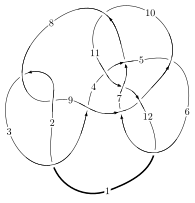
\includegraphics[width=112pt]{../../../GIT/diagram.site/Diagrams/png/2726_12n_0637.png}\\
\ \ \ A knot diagram\footnotemark}&
\allowdisplaybreaks
\textbf{Linearized knot diagam} \\
\cline{2-2}
 &
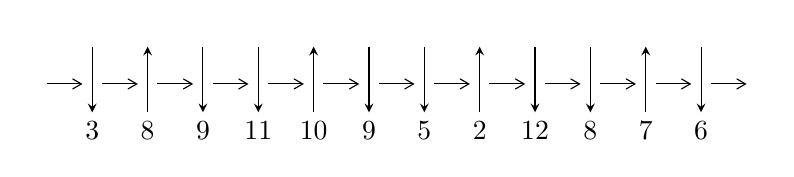
\begin{tikzpicture}[x=20pt, y=17pt]
	% nodes
	\node (C0) at (0, 0) {};
	\node (C1) at (1, 0) {};
	\node (C1U) at (1, +1) {};
	\node (C1D) at (1, -1) {3};

	\node (C2) at (2, 0) {};
	\node (C2U) at (2, +1) {};
	\node (C2D) at (2, -1) {8};

	\node (C3) at (3, 0) {};
	\node (C3U) at (3, +1) {};
	\node (C3D) at (3, -1) {9};

	\node (C4) at (4, 0) {};
	\node (C4U) at (4, +1) {};
	\node (C4D) at (4, -1) {11};

	\node (C5) at (5, 0) {};
	\node (C5U) at (5, +1) {};
	\node (C5D) at (5, -1) {10};

	\node (C6) at (6, 0) {};
	\node (C6U) at (6, +1) {};
	\node (C6D) at (6, -1) {9};

	\node (C7) at (7, 0) {};
	\node (C7U) at (7, +1) {};
	\node (C7D) at (7, -1) {5};

	\node (C8) at (8, 0) {};
	\node (C8U) at (8, +1) {};
	\node (C8D) at (8, -1) {2};

	\node (C9) at (9, 0) {};
	\node (C9U) at (9, +1) {};
	\node (C9D) at (9, -1) {12};

	\node (C10) at (10, 0) {};
	\node (C10U) at (10, +1) {};
	\node (C10D) at (10, -1) {8};

	\node (C11) at (11, 0) {};
	\node (C11U) at (11, +1) {};
	\node (C11D) at (11, -1) {7};

	\node (C12) at (12, 0) {};
	\node (C12U) at (12, +1) {};
	\node (C12D) at (12, -1) {6};
	\node (C13) at (13, 0) {};

	% arrows
	\draw[->,>={angle 60}]
	(C0) edge (C1) (C1) edge (C2) (C2) edge (C3) (C3) edge (C4) (C4) edge (C5) (C5) edge (C6) (C6) edge (C7) (C7) edge (C8) (C8) edge (C9) (C9) edge (C10) (C10) edge (C11) (C11) edge (C12) (C12) edge (C13) ;	\draw[->,>=stealth]
	(C1U) edge (C1D) (C2D) edge (C2U) (C3U) edge (C3D) (C4U) edge (C4D) (C5D) edge (C5U) (C6U) edge (C6D) (C7U) edge (C7D) (C8D) edge (C8U) (C9U) edge (C9D) (C10U) edge (C10D) (C11D) edge (C11U) (C12U) edge (C12D) ;
	\end{tikzpicture} \\
\hhline{~~} \\& 
\textbf{Solving Sequence} \\ \cline{2-2} 
 &
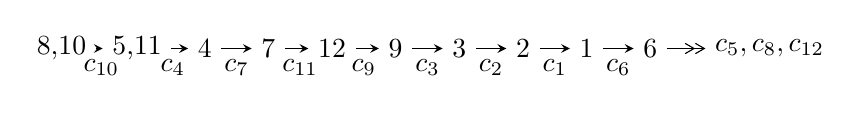
\begin{tikzpicture}[x=23pt, y=7pt]
	% node
	\node (A0) at (-1/8, 0) {8,10};
	\node (A1) at (17/16, 0) {5,11};
	\node (A2) at (17/8, 0) {4};
	\node (A3) at (25/8, 0) {7};
	\node (A4) at (33/8, 0) {12};
	\node (A5) at (41/8, 0) {9};
	\node (A6) at (49/8, 0) {3};
	\node (A7) at (57/8, 0) {2};
	\node (A8) at (65/8, 0) {1};
	\node (A9) at (73/8, 0) {6};
	\node (C1) at (1/2, -1) {$c_{10}$};
	\node (C2) at (13/8, -1) {$c_{4}$};
	\node (C3) at (21/8, -1) {$c_{7}$};
	\node (C4) at (29/8, -1) {$c_{11}$};
	\node (C5) at (37/8, -1) {$c_{9}$};
	\node (C6) at (45/8, -1) {$c_{3}$};
	\node (C7) at (53/8, -1) {$c_{2}$};
	\node (C8) at (61/8, -1) {$c_{1}$};
	\node (C9) at (69/8, -1) {$c_{6}$};
	\node (A10) at (11, 0) {$c_{5},c_{8},c_{12}$};

	% edge
	\draw[->,>=stealth]	
	(A0) edge (A1) (A1) edge (A2) (A2) edge (A3) (A3) edge (A4) (A4) edge (A5) (A5) edge (A6) (A6) edge (A7) (A7) edge (A8) (A8) edge (A9) ;
	\draw[->>,>={angle 60}]	
	(A9) edge (A10);
\end{tikzpicture} \\ 

\end{tabular} \\

\footnotetext{
The image of knot diagram is generated by the software ``\textbf{Draw programme}" developed by Andrew Bartholomew(\url{http://www.layer8.co.uk/maths/draw/index.htm\#Running-draw}), where we modified some parts for our purpose(\url{https://github.com/CATsTAILs/LinksPainter}).
}\phantom \\ \newline 
\centering \textbf{Ideals for irreducible components\footnotemark of $X_{\text{par}}$} 
 
\begin{align*}
I^u_{1}&=\langle 
-35223725986 u^{21}+30523664755 u^{20}+\cdots+210473051795 b+25821213245,\\
\phantom{I^u_{1}}&\phantom{= \langle  }740868672496 u^{21}-766689885741 u^{20}+\cdots+210473051795 a-869880690251,\\
\phantom{I^u_{1}}&\phantom{= \langle  }u^{22}- u^{21}+\cdots- u+1\rangle \\
I^u_{2}&=\langle 
3.78529\times10^{20} u^{19}-4.63105\times10^{20} u^{18}+\cdots+8.62031\times10^{21} b-2.24738\times10^{21},\\
\phantom{I^u_{2}}&\phantom{= \langle  }2.73069\times10^{22} u^{19}-2.50595\times10^{22} u^{18}+\cdots+8.62031\times10^{21} a-1.80097\times10^{23},\;u^{20}- u^{19}+\cdots-7 u+1\rangle \\
I^u_{3}&=\langle 
-3.35706\times10^{35} u^{33}-7.63609\times10^{35} u^{32}+\cdots+5.24183\times10^{36} b-4.09915\times10^{36},\\
\phantom{I^u_{3}}&\phantom{= \langle  }1.95717\times10^{37} u^{33}+4.09915\times10^{36} u^{32}+\cdots+5.24183\times10^{36} a-6.08409\times10^{37},\;u^{34}-9 u^{32}+\cdots-5 u+1\rangle \\
I^u_{4}&=\langle 
16685766983482 u^{15}+6555188230121 u^{14}+\cdots+453436720809281 b+250672039562051,\\
\phantom{I^u_{4}}&\phantom{= \langle  }-35828884147 u^{15}-26710704549 u^{14}+\cdots+766837175819 a+930772601969,\\
\phantom{I^u_{4}}&\phantom{= \langle  }u^{16}- u^{15}+\cdots-20 u+13\rangle \\
I^u_{5}&=\langle 
3.61106\times10^{67} u^{31}+1.33112\times10^{67} u^{30}+\cdots+5.05264\times10^{70} b-7.80220\times10^{69},\\
\phantom{I^u_{5}}&\phantom{= \langle  }-2.81341\times10^{59} u^{31}-1.32370\times10^{59} u^{30}+\cdots+1.01984\times10^{63} a+2.59788\times10^{62},\\
\phantom{I^u_{5}}&\phantom{= \langle  }u^{32}+u^{31}+\cdots-1290 u+1501\rangle \\
I^u_{6}&=\langle 
b- u,\;a,\;u^4+u^3+3 u^2+2 u+1\rangle \\
I^u_{7}&=\langle 
11 u^7+19 u^6+58 u^5+65 u^4-6 u^3-34 u^2+2 b+9 u-28,\;u^7+u^6+4 u^5+2 u^4-5 u^3-3 u^2+2 a+3 u-3,\\
\phantom{I^u_{7}}&\phantom{= \langle  }u^8+u^7+4 u^6+2 u^5-5 u^4-3 u^3+3 u^2-3 u+2\rangle \\
I^u_{8}&=\langle 
b,\;a+1,\;u+1\rangle \\
\\
\end{align*}
\raggedright * 8 irreducible components of $\dim_{\mathbb{C}}=0$, with total 137 representations.\\
\footnotetext{All coefficients of polynomials are rational numbers. But the coefficients are sometimes approximated in decimal forms when there is not enough margin.}
\newpage
\renewcommand{\arraystretch}{1}
\centering \section*{I. $I^u_{1}= \langle -3.52\times10^{10} u^{21}+3.05\times10^{10} u^{20}+\cdots+2.10\times10^{11} b+2.58\times10^{10},\;7.41\times10^{11} u^{21}-7.67\times10^{11} u^{20}+\cdots+2.10\times10^{11} a-8.70\times10^{11},\;u^{22}- u^{21}+\cdots- u+1 \rangle$}
\flushleft \textbf{(i) Arc colorings}\\
\begin{tabular}{m{7pt} m{180pt} m{7pt} m{180pt} }
\flushright $a_{8}=$&$\begin{pmatrix}0\\u\end{pmatrix}$ \\
\flushright $a_{10}=$&$\begin{pmatrix}1\\0\end{pmatrix}$ \\
\flushright $a_{5}=$&$\begin{pmatrix}-3.52002 u^{21}+3.64270 u^{20}+\cdots-40.0291 u+4.13298\\0.167355 u^{21}-0.145024 u^{20}+\cdots+4.64270 u-0.122682\end{pmatrix}$ \\
\flushright $a_{11}=$&$\begin{pmatrix}1\\u^2\end{pmatrix}$ \\
\flushright $a_{4}=$&$\begin{pmatrix}-3.52002 u^{21}+3.64270 u^{20}+\cdots-39.0291 u+4.13298\\0.167355 u^{21}-0.145024 u^{20}+\cdots+4.64270 u-0.122682\end{pmatrix}$ \\
\flushright $a_{7}=$&$\begin{pmatrix}-7.95997 u^{21}+8.71460 u^{20}+\cdots-67.9417 u+11.7340\\0.832645 u^{21}-0.854976 u^{20}+\cdots+13.3573 u-0.877318\end{pmatrix}$ \\
\flushright $a_{12}=$&$\begin{pmatrix}-3.13298 u^{21}+0.612962 u^{20}+\cdots-16.2045 u-19.8962\\0.122682 u^{21}+0.0446732 u^{20}+\cdots+0.612962 u+3.52002\end{pmatrix}$ \\
\flushright $a_{9}=$&$\begin{pmatrix}7.72374 u^{21}-3.11644 u^{20}+\cdots+40.9995 u+24.8315\\-0.754636 u^{21}+0.0893465 u^{20}+\cdots-3.77408 u-7.95997\end{pmatrix}$ \\
\flushright $a_{3}=$&$\begin{pmatrix}2.10661 u^{21}+3.86613 u^{20}+\cdots+4.19416 u+30.2779\\4.12150 u^{21}-5.66719 u^{20}+\cdots+21.5571 u-12.2542\end{pmatrix}$ \\
\flushright $a_{2}=$&$\begin{pmatrix}2.10661 u^{21}+3.86613 u^{20}+\cdots+4.19416 u+30.2779\\4.99760 u^{21}-7.47535 u^{20}+\cdots+25.4233 u-18.2269\end{pmatrix}$ \\
\flushright $a_{1}=$&$\begin{pmatrix}2.98797 u^{21}-0.624862 u^{20}+\cdots+15.5468 u+16.5435\\-0.145013 u^{21}-0.0118996 u^{20}+\cdots-0.657635 u-3.35266\end{pmatrix}$ \\
\flushright $a_{6}=$&$\begin{pmatrix}-3.35266 u^{21}+3.49767 u^{20}+\cdots-35.3864 u+4.01030\\0.167355 u^{21}-0.145024 u^{20}+\cdots+4.64270 u-0.122682\end{pmatrix}$\\&\end{tabular}
\flushleft \textbf{(ii) Obstruction class $= -1$}\\~\\
\flushleft \textbf{(iii) Cusp Shapes $= -\frac{1913935713454}{210473051795} u^{21}-\frac{1492818570442}{210473051795} u^{20}+\cdots-\frac{6526154909884}{210473051795} u-\frac{14593217553892}{210473051795}$}\\~\\
\newpage\renewcommand{\arraystretch}{1}
\flushleft \textbf{(iv) u-Polynomials at the component}\newline \\
\begin{tabular}{m{50pt}|m{274pt}}
Crossings & \hspace{64pt}u-Polynomials at each crossing \\
\hline $$\begin{aligned}c_{1}\end{aligned}$$&$\begin{aligned}
&u^{22}+8 u^{21}+\cdots+160 u+64
\end{aligned}$\\
\hline $$\begin{aligned}c_{2},c_{8}\end{aligned}$$&$\begin{aligned}
&u^{22}+6 u^{21}+\cdots+32 u+8
\end{aligned}$\\
\hline $$\begin{aligned}c_{3}\end{aligned}$$&$\begin{aligned}
&u^{22}-6 u^{21}+\cdots-5072 u+3880
\end{aligned}$\\
\hline $$\begin{aligned}c_{4},c_{6},c_{10}\\c_{12}\end{aligned}$$&$\begin{aligned}
&u^{22}- u^{21}+\cdots- u+1
\end{aligned}$\\
\hline $$\begin{aligned}c_{5},c_{11}\end{aligned}$$&$\begin{aligned}
&u^{22}- u^{21}+\cdots-16 u+10
\end{aligned}$\\
\hline $$\begin{aligned}c_{7},c_{9}\end{aligned}$$&$\begin{aligned}
&u^{22}-9 u^{21}+\cdots-15 u+19
\end{aligned}$\\
\hline
\end{tabular}\\~\\
\newpage\renewcommand{\arraystretch}{1}
\flushleft \textbf{(v) Riley Polynomials at the component}\newline \\
\begin{tabular}{m{50pt}|m{274pt}}
Crossings & \hspace{64pt}Riley Polynomials at each crossing \\
\hline $$\begin{aligned}c_{1}\end{aligned}$$&$\begin{aligned}
&y^{22}+12 y^{21}+\cdots+28160 y+4096
\end{aligned}$\\
\hline $$\begin{aligned}c_{2},c_{8}\end{aligned}$$&$\begin{aligned}
&y^{22}+8 y^{21}+\cdots+160 y+64
\end{aligned}$\\
\hline $$\begin{aligned}c_{3}\end{aligned}$$&$\begin{aligned}
&y^{22}+16 y^{21}+\cdots+18242976 y+15054400
\end{aligned}$\\
\hline $$\begin{aligned}c_{4},c_{6},c_{10}\\c_{12}\end{aligned}$$&$\begin{aligned}
&y^{22}+21 y^{21}+\cdots+35 y+1
\end{aligned}$\\
\hline $$\begin{aligned}c_{5},c_{11}\end{aligned}$$&$\begin{aligned}
&y^{22}+y^{21}+\cdots+624 y+100
\end{aligned}$\\
\hline $$\begin{aligned}c_{7},c_{9}\end{aligned}$$&$\begin{aligned}
&y^{22}-9 y^{21}+\cdots-187 y+361
\end{aligned}$\\
\hline
\end{tabular}\\~\\
\newpage\flushleft \textbf{(vi) Complex Volumes and Cusp Shapes}
$$\begin{array}{c|c|c}  
\text{Solutions to }I^u_{1}& \I (\text{vol} + \sqrt{-1}CS) & \text{Cusp shape}\\
 \hline 
\begin{aligned}
u &= \phantom{-}0.251396 + 1.197270 I \\
a &= -0.727101 + 0.853670 I \\
b &= \phantom{-}0.733815 - 0.410169 I\end{aligned}
 & -1.69375 - 1.58224 I & -2.92761 + 2.99168 I \\ \hline\begin{aligned}
u &= \phantom{-}0.251396 - 1.197270 I \\
a &= -0.727101 - 0.853670 I \\
b &= \phantom{-}0.733815 + 0.410169 I\end{aligned}
 & -1.69375 + 1.58224 I & -2.92761 - 2.99168 I \\ \hline\begin{aligned}
u &= -0.439138 + 1.208940 I \\
a &= -0.366754 + 0.753125 I \\
b &= \phantom{-}0.825819 + 0.642867 I\end{aligned}
 & \phantom{-}7.22176 + 4.64537 I & -1.48411 - 2.36378 I \\ \hline\begin{aligned}
u &= -0.439138 - 1.208940 I \\
a &= -0.366754 - 0.753125 I \\
b &= \phantom{-}0.825819 - 0.642867 I\end{aligned}
 & \phantom{-}7.22176 - 4.64537 I & -1.48411 + 2.36378 I \\ \hline\begin{aligned}
u &= -0.100425 + 0.610392 I \\
a &= -0.598286 - 0.326486 I \\
b &= \phantom{-}0.076424 + 0.802089 I\end{aligned}
 & -0.049452 + 1.407930 I & -0.88049 - 5.93296 I \\ \hline\begin{aligned}
u &= -0.100425 - 0.610392 I \\
a &= -0.598286 + 0.326486 I \\
b &= \phantom{-}0.076424 - 0.802089 I\end{aligned}
 & -0.049452 - 1.407930 I & -0.88049 + 5.93296 I \\ \hline\begin{aligned}
u &= \phantom{-}0.311341 + 1.349370 I \\
a &= \phantom{-}0.386640 + 0.716640 I \\
b &= -0.957311 + 0.438847 I\end{aligned}
 & \phantom{-}8.03816 + 1.82472 I & -0.36555 - 2.90365 I \\ \hline\begin{aligned}
u &= \phantom{-}0.311341 - 1.349370 I \\
a &= \phantom{-}0.386640 - 0.716640 I \\
b &= -0.957311 - 0.438847 I\end{aligned}
 & \phantom{-}8.03816 - 1.82472 I & -0.36555 + 2.90365 I \\ \hline\begin{aligned}
u &= \phantom{-}0.70785 + 1.27677 I \\
a &= -0.942108 + 0.435063 I \\
b &= \phantom{-}0.985198 - 0.917340 I\end{aligned}
 & -2.15736 - 11.05600 I & -5.86304 + 8.74726 I \\ \hline\begin{aligned}
u &= \phantom{-}0.70785 - 1.27677 I \\
a &= -0.942108 - 0.435063 I \\
b &= \phantom{-}0.985198 + 0.917340 I\end{aligned}
 & -2.15736 + 11.05600 I & -5.86304 - 8.74726 I\\
 \hline 
 \end{array}$$\newpage$$\begin{array}{c|c|c}  
\text{Solutions to }I^u_{1}& \I (\text{vol} + \sqrt{-1}CS) & \text{Cusp shape}\\
 \hline 
\begin{aligned}
u &= -0.43272 + 1.42172 I \\
a &= \phantom{-}0.745026 + 0.586778 I \\
b &= -1.077150 - 0.571146 I\end{aligned}
 & \phantom{-}2.42448 + 6.49307 I & -0.75771 - 5.60630 I \\ \hline\begin{aligned}
u &= -0.43272 - 1.42172 I \\
a &= \phantom{-}0.745026 - 0.586778 I \\
b &= -1.077150 + 0.571146 I\end{aligned}
 & \phantom{-}2.42448 - 6.49307 I & -0.75771 + 5.60630 I \\ \hline\begin{aligned}
u &= -0.131155 + 0.475245 I \\
a &= -1.59000 - 1.04889 I \\
b &= \phantom{-}0.069853 + 0.892314 I\end{aligned}
 & -0.69331 + 1.97766 I & -2.32963 - 3.06093 I \\ \hline\begin{aligned}
u &= -0.131155 - 0.475245 I \\
a &= -1.59000 + 1.04889 I \\
b &= \phantom{-}0.069853 - 0.892314 I\end{aligned}
 & -0.69331 - 1.97766 I & -2.32963 + 3.06093 I \\ \hline\begin{aligned}
u &= \phantom{-}0.145985 + 0.422253 I \\
a &= \phantom{-}2.38098 - 1.30459 I \\
b &= -0.066959 + 0.920596 I\end{aligned}
 & -2.79098 - 6.48658 I & -4.59769 + 4.99587 I \\ \hline\begin{aligned}
u &= \phantom{-}0.145985 - 0.422253 I \\
a &= \phantom{-}2.38098 + 1.30459 I \\
b &= -0.066959 - 0.920596 I\end{aligned}
 & -2.79098 + 6.48658 I & -4.59769 - 4.99587 I \\ \hline\begin{aligned}
u &= \phantom{-}0.062233 + 0.424223 I \\
a &= \phantom{-}1.23180 - 2.37884 I \\
b &= -0.029071 + 0.908159 I\end{aligned}
 & -4.30511 + 0.52403 I & -12.36500 - 2.34222 I \\ \hline\begin{aligned}
u &= \phantom{-}0.062233 - 0.424223 I \\
a &= \phantom{-}1.23180 + 2.37884 I \\
b &= -0.029071 - 0.908159 I\end{aligned}
 & -4.30511 - 0.52403 I & -12.36500 + 2.34222 I \\ \hline\begin{aligned}
u &= -1.05080 + 1.58014 I \\
a &= \phantom{-}0.749692 + 0.219224 I \\
b &= -1.36686 - 1.21476 I\end{aligned}
 & \phantom{-}7.00864 + 11.78040 I & -2.49367 - 5.42252 I \\ \hline\begin{aligned}
u &= -1.05080 - 1.58014 I \\
a &= \phantom{-}0.749692 - 0.219224 I \\
b &= -1.36686 + 1.21476 I\end{aligned}
 & \phantom{-}7.00864 - 11.78040 I & -2.49367 + 5.42252 I\\
 \hline 
 \end{array}$$\newpage$$\begin{array}{c|c|c}  
\text{Solutions to }I^u_{1}& \I (\text{vol} + \sqrt{-1}CS) & \text{Cusp shape}\\
 \hline 
\begin{aligned}
u &= \phantom{-}1.17544 + 1.50294 I \\
a &= -0.769890 + 0.154115 I \\
b &= \phantom{-}1.30624 - 1.35244 I\end{aligned}
 & \phantom{-}5.9137 - 18.4120 I & -4.00000 + 9.61591 I \\ \hline\begin{aligned}
u &= \phantom{-}1.17544 - 1.50294 I \\
a &= -0.769890 - 0.154115 I \\
b &= \phantom{-}1.30624 + 1.35244 I\end{aligned}
 & \phantom{-}5.9137 + 18.4120 I & -4.00000 - 9.61591 I\\
 \hline 
 \end{array}$$\newpage\newpage\renewcommand{\arraystretch}{1}
\centering \section*{II. $I^u_{2}= \langle 3.79\times10^{20} u^{19}-4.63\times10^{20} u^{18}+\cdots+8.62\times10^{21} b-2.25\times10^{21},\;2.73\times10^{22} u^{19}-2.51\times10^{22} u^{18}+\cdots+8.62\times10^{21} a-1.80\times10^{23},\;u^{20}- u^{19}+\cdots-7 u+1 \rangle$}
\flushleft \textbf{(i) Arc colorings}\\
\begin{tabular}{m{7pt} m{180pt} m{7pt} m{180pt} }
\flushright $a_{8}=$&$\begin{pmatrix}0\\u\end{pmatrix}$ \\
\flushright $a_{10}=$&$\begin{pmatrix}1\\0\end{pmatrix}$ \\
\flushright $a_{5}=$&$\begin{pmatrix}-3.16774 u^{19}+2.90704 u^{18}+\cdots+10.9832 u+20.8921\\-0.0439113 u^{19}+0.0537225 u^{18}+\cdots+2.34279 u+0.260708\end{pmatrix}$ \\
\flushright $a_{11}=$&$\begin{pmatrix}1\\u^2\end{pmatrix}$ \\
\flushright $a_{4}=$&$\begin{pmatrix}-3.16774 u^{19}+2.90704 u^{18}+\cdots+11.9832 u+20.8921\\-0.0439113 u^{19}+0.0537225 u^{18}+\cdots+2.34279 u+0.260708\end{pmatrix}$ \\
\flushright $a_{7}=$&$\begin{pmatrix}-8.81122 u^{19}+7.79546 u^{18}+\cdots-18.5918 u+54.1639\\-0.175015 u^{19}+0.186912 u^{18}+\cdots+4.04373 u+1.27646\end{pmatrix}$ \\
\flushright $a_{12}=$&$\begin{pmatrix}3.92566 u^{19}-3.36351 u^{18}+\cdots+33.8425 u-29.7066\\0.0217085 u^{19}-0.0143026 u^{18}+\cdots+0.00468521 u-0.781074\end{pmatrix}$ \\
\flushright $a_{9}=$&$\begin{pmatrix}2.88820 u^{19}-2.46456 u^{18}+\cdots+26.3232 u-20.1143\\0.0364007 u^{19}-0.0247875 u^{18}+\cdots+0.0259089 u-0.598653\end{pmatrix}$ \\
\flushright $a_{3}=$&$\begin{pmatrix}1.64440 u^{19}-1.25672 u^{18}+\cdots+38.9478 u-7.71164\\0.0771122 u^{19}-0.0734388 u^{18}+\cdots+0.753454 u-0.595866\end{pmatrix}$ \\
\flushright $a_{2}=$&$\begin{pmatrix}1.64440 u^{19}-1.25672 u^{18}+\cdots+38.9478 u-7.71164\\0.122553 u^{19}-0.0983998 u^{18}+\cdots+1.82280 u-0.983543\end{pmatrix}$ \\
\flushright $a_{1}=$&$\begin{pmatrix}1.28627 u^{19}-1.10467 u^{18}+\cdots+8.75002 u-13.9350\\-0.0118974 u^{19}+0.0110797 u^{18}+\cdots-0.0513570 u-0.175015\end{pmatrix}$ \\
\flushright $a_{6}=$&$\begin{pmatrix}-3.21165 u^{19}+2.96076 u^{18}+\cdots+13.3259 u+21.1528\\-0.0439113 u^{19}+0.0537225 u^{18}+\cdots+2.34279 u+0.260708\end{pmatrix}$\\&\end{tabular}
\flushleft \textbf{(ii) Obstruction class $= -1$}\\~\\
\flushleft \textbf{(iii) Cusp Shapes $= -\frac{97906072790078772930140}{8620310934921930687151} u^{19}+\frac{81524634991414853459581}{8620310934921930687151} u^{18}+\cdots-\frac{1059865978912088574268036}{8620310934921930687151} u+\frac{616271317183349139490199}{8620310934921930687151}$}\\~\\
\newpage\renewcommand{\arraystretch}{1}
\flushleft \textbf{(iv) u-Polynomials at the component}\newline \\
\begin{tabular}{m{50pt}|m{274pt}}
Crossings & \hspace{64pt}u-Polynomials at each crossing \\
\hline $$\begin{aligned}c_{1}\end{aligned}$$&$\begin{aligned}
&(u^{10}+4 u^9+\cdots-12 u+16)^{2}
\end{aligned}$\\
\hline $$\begin{aligned}c_{2},c_{8}\end{aligned}$$&$\begin{aligned}
&(u^{10}+4 u^9+10 u^8+16 u^7+19 u^6+15 u^5+6 u^4-5 u^3-11 u^2-10 u-4)^{2}
\end{aligned}$\\
\hline $$\begin{aligned}c_{3}\end{aligned}$$&$\begin{aligned}
&(u^{10}-4 u^9+\cdots-66 u-52)^{2}
\end{aligned}$\\
\hline $$\begin{aligned}c_{4},c_{6},c_{10}\\c_{12}\end{aligned}$$&$\begin{aligned}
&u^{20}- u^{19}+\cdots-7 u+1
\end{aligned}$\\
\hline $$\begin{aligned}c_{5},c_{11}\end{aligned}$$&$\begin{aligned}
&(u^{10}-4 u^8- u^7+10 u^6+3 u^5-12 u^4-4 u^3+6 u^2+u-1)^2
\end{aligned}$\\
\hline $$\begin{aligned}c_{7},c_{9}\end{aligned}$$&$\begin{aligned}
&u^{20}-7 u^{19}+\cdots+710 u-71
\end{aligned}$\\
\hline
\end{tabular}\\~\\
\newpage\renewcommand{\arraystretch}{1}
\flushleft \textbf{(v) Riley Polynomials at the component}\newline \\
\begin{tabular}{m{50pt}|m{274pt}}
Crossings & \hspace{64pt}Riley Polynomials at each crossing \\
\hline $$\begin{aligned}c_{1}\end{aligned}$$&$\begin{aligned}
&(y^{10}+4 y^9+\cdots-1008 y+256)^{2}
\end{aligned}$\\
\hline $$\begin{aligned}c_{2},c_{8}\end{aligned}$$&$\begin{aligned}
&(y^{10}+4 y^9+\cdots-12 y+16)^{2}
\end{aligned}$\\
\hline $$\begin{aligned}c_{3}\end{aligned}$$&$\begin{aligned}
&(y^{10}+4 y^9+\cdots-14028 y+2704)^{2}
\end{aligned}$\\
\hline $$\begin{aligned}c_{4},c_{6},c_{10}\\c_{12}\end{aligned}$$&$\begin{aligned}
&y^{20}+3 y^{19}+\cdots-77 y+1
\end{aligned}$\\
\hline $$\begin{aligned}c_{5},c_{11}\end{aligned}$$&$\begin{aligned}
&(y^{10}-8 y^9+\cdots-13 y+1)^{2}
\end{aligned}$\\
\hline $$\begin{aligned}c_{7},c_{9}\end{aligned}$$&$\begin{aligned}
&y^{20}-7 y^{19}+\cdots-29394 y+5041
\end{aligned}$\\
\hline
\end{tabular}\\~\\
\newpage\flushleft \textbf{(vi) Complex Volumes and Cusp Shapes}
$$\begin{array}{c|c|c}  
\text{Solutions to }I^u_{2}& \I (\text{vol} + \sqrt{-1}CS) & \text{Cusp shape}\\
 \hline 
\begin{aligned}
u &= \phantom{-}0.606294 + 1.022320 I \\
a &= \phantom{-}0.506435 + 1.185730 I \\
b &= -1.20672 + 0.84674 I\end{aligned}
 & \phantom{-}6.80818 - 10.55520 I & -2.80651 + 7.76192 I \\ \hline\begin{aligned}
u &= \phantom{-}0.606294 - 1.022320 I \\
a &= \phantom{-}0.506435 - 1.185730 I \\
b &= -1.20672 - 0.84674 I\end{aligned}
 & \phantom{-}6.80818 + 10.55520 I & -2.80651 - 7.76192 I \\ \hline\begin{aligned}
u &= \phantom{-}0.410689 + 1.146110 I \\
a &= -0.911522 + 0.251562 I \\
b &= \phantom{-}1.21747\phantom{ +0.000000I}\end{aligned}
 & \phantom{-}3.96203\phantom{ +0.000000I} & \phantom{-}1.71627 + 0. I\phantom{ +0.000000I} \\ \hline\begin{aligned}
u &= \phantom{-}0.410689 - 1.146110 I \\
a &= -0.911522 - 0.251562 I \\
b &= \phantom{-}1.21747\phantom{ +0.000000I}\end{aligned}
 & \phantom{-}3.96203\phantom{ +0.000000I} & \phantom{-}1.71627 + 0. I\phantom{ +0.000000I} \\ \hline\begin{aligned}
u &= -0.447983 + 1.156950 I \\
a &= -0.650705 + 0.989358 I \\
b &= \phantom{-}1.31797 + 0.70573 I\end{aligned}
 & \phantom{-}7.99409 + 4.11330 I & -0.72706 - 2.84018 I \\ \hline\begin{aligned}
u &= -0.447983 - 1.156950 I \\
a &= -0.650705 - 0.989358 I \\
b &= \phantom{-}1.31797 - 0.70573 I\end{aligned}
 & \phantom{-}7.99409 - 4.11330 I & -0.72706 + 2.84018 I \\ \hline\begin{aligned}
u &= -0.050609 + 0.749544 I \\
a &= \phantom{-}1.71190 + 0.54431 I \\
b &= -0.966704 + 0.315261 I\end{aligned}
 & -0.07213 - 3.52780 I & -2.13233 + 4.34006 I \\ \hline\begin{aligned}
u &= -0.050609 - 0.749544 I \\
a &= \phantom{-}1.71190 - 0.54431 I \\
b &= -0.966704 - 0.315261 I\end{aligned}
 & -0.07213 + 3.52780 I & -2.13233 - 4.34006 I \\ \hline\begin{aligned}
u &= -0.884394 + 1.054470 I \\
a &= \phantom{-}0.719695 + 0.083108 I \\
b &= -0.966704 - 0.315261 I\end{aligned}
 & -0.07213 + 3.52780 I & -2.13233 - 4.34006 I \\ \hline\begin{aligned}
u &= -0.884394 - 1.054470 I \\
a &= \phantom{-}0.719695 - 0.083108 I \\
b &= -0.966704 + 0.315261 I\end{aligned}
 & -0.07213 - 3.52780 I & -2.13233 + 4.34006 I\\
 \hline 
 \end{array}$$\newpage$$\begin{array}{c|c|c}  
\text{Solutions to }I^u_{2}& \I (\text{vol} + \sqrt{-1}CS) & \text{Cusp shape}\\
 \hline 
\begin{aligned}
u &= -1.53443\phantom{ +0.000000I} \\
a &= \phantom{-}0.408700\phantom{ +0.000000I} \\
b &= -0.572155\phantom{ +0.000000I}\end{aligned}
 & -3.24417\phantom{ +0.000000I} & \phantom{-}9.61450\phantom{ +0.000000I} \\ \hline\begin{aligned}
u &= \phantom{-}1.70396 + 0.20280 I \\
a &= -0.406335 + 0.011690 I \\
b &= \phantom{-}0.532805 - 0.044567 I\end{aligned}
 & -6.86440 - 4.53571 I & \phantom{-}10.5005 + 34.9465 I \\ \hline\begin{aligned}
u &= \phantom{-}1.70396 - 0.20280 I \\
a &= -0.406335 - 0.011690 I \\
b &= \phantom{-}0.532805 + 0.044567 I\end{aligned}
 & -6.86440 + 4.53571 I & \phantom{-}10.5005 - 34.9465 I \\ \hline\begin{aligned}
u &= -0.213343\phantom{ +0.000000I} \\
a &= -7.88331\phantom{ +0.000000I} \\
b &= -0.572155\phantom{ +0.000000I}\end{aligned}
 & -3.24417\phantom{ +0.000000I} & \phantom{-}9.61450\phantom{ +0.000000I} \\ \hline\begin{aligned}
u &= \phantom{-}1.03765 + 1.47270 I \\
a &= -0.661123 + 0.144524 I \\
b &= \phantom{-}1.31797 - 0.70573 I\end{aligned}
 & \phantom{-}7.99409 - 4.11330 I & -0.72706 + 2.84018 I \\ \hline\begin{aligned}
u &= \phantom{-}1.03765 - 1.47270 I \\
a &= -0.661123 - 0.144524 I \\
b &= \phantom{-}1.31797 + 0.70573 I\end{aligned}
 & \phantom{-}7.99409 + 4.11330 I & -0.72706 - 2.84018 I \\ \hline\begin{aligned}
u &= -1.16158 + 1.41196 I \\
a &= \phantom{-}0.665605 + 0.116987 I \\
b &= -1.20672 - 0.84674 I\end{aligned}
 & \phantom{-}6.80818 + 10.55520 I & -2.80651 - 7.76192 I \\ \hline\begin{aligned}
u &= -1.16158 - 1.41196 I \\
a &= \phantom{-}0.665605 - 0.116987 I \\
b &= -1.20672 + 0.84674 I\end{aligned}
 & \phantom{-}6.80818 - 10.55520 I & -2.80651 + 7.76192 I \\ \hline\begin{aligned}
u &= \phantom{-}0.159854 + 0.046896 I \\
a &= \phantom{-}11.26340 - 7.33066 I \\
b &= \phantom{-}0.532805 + 0.044567 I\end{aligned}
 & -6.86440 + 4.53571 I & \phantom{-}10.5005 - 34.9465 I \\ \hline\begin{aligned}
u &= \phantom{-}0.159854 - 0.046896 I \\
a &= \phantom{-}11.26340 + 7.33066 I \\
b &= \phantom{-}0.532805 - 0.044567 I\end{aligned}
 & -6.86440 - 4.53571 I & \phantom{-}10.5005 + 34.9465 I\\
 \hline 
 \end{array}$$\newpage\newpage\renewcommand{\arraystretch}{1}
\centering \section*{III. $I^u_{3}= \langle -3.36\times10^{35} u^{33}-7.64\times10^{35} u^{32}+\cdots+5.24\times10^{36} b-4.10\times10^{36},\;1.96\times10^{37} u^{33}+4.10\times10^{36} u^{32}+\cdots+5.24\times10^{36} a-6.08\times10^{37},\;u^{34}-9 u^{32}+\cdots-5 u+1 \rangle$}
\flushleft \textbf{(i) Arc colorings}\\
\begin{tabular}{m{7pt} m{180pt} m{7pt} m{180pt} }
\flushright $a_{8}=$&$\begin{pmatrix}0\\u\end{pmatrix}$ \\
\flushright $a_{10}=$&$\begin{pmatrix}1\\0\end{pmatrix}$ \\
\flushright $a_{5}=$&$\begin{pmatrix}-3.73375 u^{33}-0.782006 u^{32}+\cdots-25.6210 u+11.6068\\0.0640435 u^{33}+0.145676 u^{32}+\cdots-1.17628 u+0.782006\end{pmatrix}$ \\
\flushright $a_{11}=$&$\begin{pmatrix}1\\u^2\end{pmatrix}$ \\
\flushright $a_{4}=$&$\begin{pmatrix}-3.73375 u^{33}-0.782006 u^{32}+\cdots-26.6210 u+11.6068\\0.0640435 u^{33}+0.145676 u^{32}+\cdots-1.17628 u+0.782006\end{pmatrix}$ \\
\flushright $a_{7}=$&$\begin{pmatrix}-8.90770 u^{33}-2.14572 u^{32}+\cdots-71.2828 u+27.4824\\-0.376603 u^{33}+0.0354177 u^{32}+\cdots-0.644601 u+1.36371\end{pmatrix}$ \\
\flushright $a_{12}=$&$\begin{pmatrix}-4.42221 u^{33}-0.993348 u^{32}+\cdots-37.1005 u+14.3537\\-0.0610815 u^{33}-0.112187 u^{32}+\cdots+1.07701 u+0.552701\end{pmatrix}$ \\
\flushright $a_{9}=$&$\begin{pmatrix}3.06716 u^{33}+0.825714 u^{32}+\cdots+27.3561 u-9.54342\\0.232957 u^{33}+0.180886 u^{32}+\cdots-1.92567 u-0.0777394\end{pmatrix}$ \\
\flushright $a_{3}=$&$\begin{pmatrix}1.55716 u^{33}+0.844911 u^{32}+\cdots+11.9349 u-1.31495\\-0.0686076 u^{33}-0.182006 u^{32}+\cdots+3.42735 u-1.07782\end{pmatrix}$ \\
\flushright $a_{2}=$&$\begin{pmatrix}1.55716 u^{33}+0.844911 u^{32}+\cdots+11.9349 u-1.31495\\0.202905 u^{33}-0.0632946 u^{32}+\cdots+6.09474 u-1.92273\end{pmatrix}$ \\
\flushright $a_{1}=$&$\begin{pmatrix}2.08828 u^{33}+0.392969 u^{32}+\cdots+13.8037 u-7.12091\\0.0856981 u^{33}-0.102474 u^{32}+\cdots+2.98707 u-0.747975\end{pmatrix}$ \\
\flushright $a_{6}=$&$\begin{pmatrix}-3.66970 u^{33}-0.636330 u^{32}+\cdots-26.7973 u+12.3888\\0.0640435 u^{33}+0.145676 u^{32}+\cdots-1.17628 u+0.782006\end{pmatrix}$\\&\end{tabular}
\flushleft \textbf{(ii) Obstruction class $= 1$}\\~\\
\flushleft \textbf{(iii) Cusp Shapes $= 20.8441 u^{33}+4.37870 u^{32}+\cdots+173.006 u-75.6418$}\\~\\
\newpage\renewcommand{\arraystretch}{1}
\flushleft \textbf{(iv) u-Polynomials at the component}\newline \\
\begin{tabular}{m{50pt}|m{274pt}}
Crossings & \hspace{64pt}u-Polynomials at each crossing \\
\hline $$\begin{aligned}c_{1}\end{aligned}$$&$\begin{aligned}
&(u^{17}-8 u^{16}+\cdots-11 u+2)^{2}
\end{aligned}$\\
\hline $$\begin{aligned}c_{2},c_{8}\end{aligned}$$&$\begin{aligned}
&u^{34}+8 u^{32}+\cdots-11 u^2-2
\end{aligned}$\\
\hline $$\begin{aligned}c_{3}\end{aligned}$$&$\begin{aligned}
&u^{34}+12 u^{32}+\cdots-99 u^2-2
\end{aligned}$\\
\hline $$\begin{aligned}c_{4},c_{10}\end{aligned}$$&$\begin{aligned}
&u^{34}-9 u^{32}+\cdots-5 u+1
\end{aligned}$\\
\hline $$\begin{aligned}c_{5},c_{11}\end{aligned}$$&$\begin{aligned}
&u^{34}+3 u^{32}+\cdots+31 u^2-2
\end{aligned}$\\
\hline $$\begin{aligned}c_{6},c_{12}\end{aligned}$$&$\begin{aligned}
&u^{34}-9 u^{32}+\cdots+5 u+1
\end{aligned}$\\
\hline $$\begin{aligned}c_{7}\end{aligned}$$&$\begin{aligned}
&u^{34}+18 u^{33}+\cdots+10 u+1
\end{aligned}$\\
\hline $$\begin{aligned}c_{9}\end{aligned}$$&$\begin{aligned}
&u^{34}-18 u^{33}+\cdots-10 u+1
\end{aligned}$\\
\hline
\end{tabular}\\~\\
\newpage\renewcommand{\arraystretch}{1}
\flushleft \textbf{(v) Riley Polynomials at the component}\newline \\
\begin{tabular}{m{50pt}|m{274pt}}
Crossings & \hspace{64pt}Riley Polynomials at each crossing \\
\hline $$\begin{aligned}c_{1}\end{aligned}$$&$\begin{aligned}
&(y^{17}+10 y^{16}+\cdots-11 y-4)^{2}
\end{aligned}$\\
\hline $$\begin{aligned}c_{2},c_{8}\end{aligned}$$&$\begin{aligned}
&(y^{17}+8 y^{16}+\cdots-11 y-2)^{2}
\end{aligned}$\\
\hline $$\begin{aligned}c_{3}\end{aligned}$$&$\begin{aligned}
&(y^{17}+12 y^{16}+\cdots-99 y-2)^{2}
\end{aligned}$\\
\hline $$\begin{aligned}c_{4},c_{6},c_{10}\\c_{12}\end{aligned}$$&$\begin{aligned}
&y^{34}-18 y^{33}+\cdots-5 y+1
\end{aligned}$\\
\hline $$\begin{aligned}c_{5},c_{11}\end{aligned}$$&$\begin{aligned}
&(y^{17}+3 y^{16}+\cdots+31 y-2)^{2}
\end{aligned}$\\
\hline $$\begin{aligned}c_{7},c_{9}\end{aligned}$$&$\begin{aligned}
&y^{34}-14 y^{33}+\cdots-4 y+1
\end{aligned}$\\
\hline
\end{tabular}\\~\\
\newpage\flushleft \textbf{(vi) Complex Volumes and Cusp Shapes}
$$\begin{array}{c|c|c}  
\text{Solutions to }I^u_{3}& \I (\text{vol} + \sqrt{-1}CS) & \text{Cusp shape}\\
 \hline 
\begin{aligned}
u &= \phantom{-}0.948002 + 0.313646 I \\
a &= \phantom{-}1.49270 + 0.75341 I \\
b &= -0.201379 + 1.177010 I\end{aligned}
 & -3.90984 - 7.35529 I & -10.7026 + 11.0707 I \\ \hline\begin{aligned}
u &= \phantom{-}0.948002 - 0.313646 I \\
a &= \phantom{-}1.49270 - 0.75341 I \\
b &= -0.201379 - 1.177010 I\end{aligned}
 & -3.90984 + 7.35529 I & -10.7026 - 11.0707 I \\ \hline\begin{aligned}
u &= \phantom{-}0.956410 + 0.604090 I \\
a &= \phantom{-}1.388120 + 0.148389 I \\
b &= -0.364697 + 1.081480 I\end{aligned}
 & -4.51641 - 1.30867 I & -12.27157 + 0.31860 I \\ \hline\begin{aligned}
u &= \phantom{-}0.956410 - 0.604090 I \\
a &= \phantom{-}1.388120 - 0.148389 I \\
b &= -0.364697 - 1.081480 I\end{aligned}
 & -4.51641 + 1.30867 I & -12.27157 - 0.31860 I \\ \hline\begin{aligned}
u &= \phantom{-}0.301826 + 0.794742 I \\
a &= -0.242452 + 0.645424 I \\
b &= -0.480417 - 1.259920 I\end{aligned}
 & -3.12305 + 4.90974 I & -4.98224 - 0.13853 I \\ \hline\begin{aligned}
u &= \phantom{-}0.301826 - 0.794742 I \\
a &= -0.242452 - 0.645424 I \\
b &= -0.480417 + 1.259920 I\end{aligned}
 & -3.12305 - 4.90974 I & -4.98224 + 0.13853 I \\ \hline\begin{aligned}
u &= -1.127990 + 0.273851 I \\
a &= -1.138540 + 0.718861 I \\
b &= \phantom{-}0.208856 + 1.290280 I\end{aligned}
 & -2.73299 + 3.07671 I & -3.59376 - 6.57908 I \\ \hline\begin{aligned}
u &= -1.127990 - 0.273851 I \\
a &= -1.138540 - 0.718861 I \\
b &= \phantom{-}0.208856 - 1.290280 I\end{aligned}
 & -2.73299 - 3.07671 I & -3.59376 + 6.57908 I \\ \hline\begin{aligned}
u &= -0.070405 + 0.815044 I \\
a &= \phantom{-}0.532860 + 0.628017 I \\
b &= -0.208856 - 1.290280 I\end{aligned}
 & -2.73299 + 3.07671 I & -3.59376 - 6.57908 I \\ \hline\begin{aligned}
u &= -0.070405 - 0.815044 I \\
a &= \phantom{-}0.532860 - 0.628017 I \\
b &= -0.208856 + 1.290280 I\end{aligned}
 & -2.73299 - 3.07671 I & -3.59376 + 6.57908 I\\
 \hline 
 \end{array}$$\newpage$$\begin{array}{c|c|c}  
\text{Solutions to }I^u_{3}& \I (\text{vol} + \sqrt{-1}CS) & \text{Cusp shape}\\
 \hline 
\begin{aligned}
u &= \phantom{-}0.251748 + 1.192390 I \\
a &= \phantom{-}1.025750 - 0.598178 I \\
b &= -1.286020 + 0.236008 I\end{aligned}
 & \phantom{-}4.34137 - 0.62662 I & \phantom{-}0.702844 + 0.664865 I \\ \hline\begin{aligned}
u &= \phantom{-}0.251748 - 1.192390 I \\
a &= \phantom{-}1.025750 + 0.598178 I \\
b &= -1.286020 - 0.236008 I\end{aligned}
 & \phantom{-}4.34137 + 0.62662 I & \phantom{-}0.702844 - 0.664865 I \\ \hline\begin{aligned}
u &= -1.044090 + 0.683860 I \\
a &= -0.761913 + 0.166704 I \\
b &= \phantom{-}0.807885 + 0.507938 I\end{aligned}
 & -1.39035 + 4.13256 I & -8.96641 - 7.21181 I \\ \hline\begin{aligned}
u &= -1.044090 - 0.683860 I \\
a &= -0.761913 - 0.166704 I \\
b &= \phantom{-}0.807885 - 0.507938 I\end{aligned}
 & -1.39035 - 4.13256 I & -8.96641 + 7.21181 I \\ \hline\begin{aligned}
u &= \phantom{-}0.647873 + 0.299417 I \\
a &= \phantom{-}1.00359 + 1.26631 I \\
b &= -0.807885 + 0.507938 I\end{aligned}
 & -1.39035 - 4.13256 I & -8.96641 + 7.21181 I \\ \hline\begin{aligned}
u &= \phantom{-}0.647873 - 0.299417 I \\
a &= \phantom{-}1.00359 - 1.26631 I \\
b &= -0.807885 - 0.507938 I\end{aligned}
 & -1.39035 + 4.13256 I & -8.96641 - 7.21181 I \\ \hline\begin{aligned}
u &= -1.199710 + 0.613641 I \\
a &= -1.068440 + 0.282667 I \\
b &= \phantom{-}0.480417 + 1.259920 I\end{aligned}
 & -3.12305 + 4.90974 I & -4.98224 + 0. I\phantom{ +0.000000I} \\ \hline\begin{aligned}
u &= -1.199710 - 0.613641 I \\
a &= -1.068440 - 0.282667 I \\
b &= \phantom{-}0.480417 - 1.259920 I\end{aligned}
 & -3.12305 - 4.90974 I & -4.98224 + 0. I\phantom{ +0.000000I} \\ \hline\begin{aligned}
u &= \phantom{-}0.067240 + 0.640701 I \\
a &= -0.90142 + 1.12971 I \\
b &= \phantom{-}0.201379 - 1.177010 I\end{aligned}
 & -3.90984 - 7.35529 I & -10.7026 + 11.0707 I \\ \hline\begin{aligned}
u &= \phantom{-}0.067240 - 0.640701 I \\
a &= -0.90142 - 1.12971 I \\
b &= \phantom{-}0.201379 + 1.177010 I\end{aligned}
 & -3.90984 + 7.35529 I & -10.7026 - 11.0707 I\\
 \hline 
 \end{array}$$\newpage$$\begin{array}{c|c|c}  
\text{Solutions to }I^u_{3}& \I (\text{vol} + \sqrt{-1}CS) & \text{Cusp shape}\\
 \hline 
\begin{aligned}
u &= -0.504150 + 1.265790 I \\
a &= -0.961784 - 0.364583 I \\
b &= \phantom{-}1.335370 + 0.453210 I\end{aligned}
 & \phantom{-}4.40017 + 6.90997 I & \phantom{-0.000000 } 0. - 5.88125 I \\ \hline\begin{aligned}
u &= -0.504150 - 1.265790 I \\
a &= -0.961784 + 0.364583 I \\
b &= \phantom{-}1.335370 - 0.453210 I\end{aligned}
 & \phantom{-}4.40017 - 6.90997 I & \phantom{-0.000000 -}0. + 5.88125 I \\ \hline\begin{aligned}
u &= -0.604342\phantom{ +0.000000I} \\
a &= -2.59153\phantom{ +0.000000I} \\
b &= -0.342161\phantom{ +0.000000I}\end{aligned}
 & -3.55226\phantom{ +0.000000I} & -16.8940\phantom{ +0.000000I} \\ \hline\begin{aligned}
u &= -1.39868\phantom{ +0.000000I} \\
a &= -0.540058\phantom{ +0.000000I} \\
b &= \phantom{-}0.342161\phantom{ +0.000000I}\end{aligned}
 & -3.55226\phantom{ +0.000000I} & -16.8940\phantom{ +0.000000I} \\ \hline\begin{aligned}
u &= -0.179282 + 0.553299 I \\
a &= \phantom{-}0.47174 + 1.58611 I \\
b &= \phantom{-}0.364697 - 1.081480 I\end{aligned}
 & -4.51641 - 1.30867 I & -12.27157 + 0.31860 I \\ \hline\begin{aligned}
u &= -0.179282 - 0.553299 I \\
a &= \phantom{-}0.47174 - 1.58611 I \\
b &= \phantom{-}0.364697 + 1.081480 I\end{aligned}
 & -4.51641 + 1.30867 I & -12.27157 - 0.31860 I \\ \hline\begin{aligned}
u &= \phantom{-}1.56336 + 0.01828 I \\
a &= \phantom{-}0.097753 + 0.190650 I \\
b &= -1.335370 + 0.453210 I\end{aligned}
 & \phantom{-}4.40017 - 6.90997 I & \phantom{-0.000000 -}0. + 5.88125 I \\ \hline\begin{aligned}
u &= \phantom{-}1.56336 - 0.01828 I \\
a &= \phantom{-}0.097753 - 0.190650 I \\
b &= -1.335370 - 0.453210 I\end{aligned}
 & \phantom{-}4.40017 + 6.90997 I & \phantom{-0.000000 } 0. - 5.88125 I \\ \hline\begin{aligned}
u &= \phantom{-}0.329313 + 0.165692 I \\
a &= \phantom{-}4.37347 - 4.17301 I \\
b &= \phantom{-}0.480307 - 0.026404 I\end{aligned}
 & -6.91964 + 4.44078 I & -26.1531 + 27.7299 I \\ \hline\begin{aligned}
u &= \phantom{-}0.329313 - 0.165692 I \\
a &= \phantom{-}4.37347 + 4.17301 I \\
b &= \phantom{-}0.480307 + 0.026404 I\end{aligned}
 & -6.91964 - 4.44078 I & -26.1531 - 27.7299 I\\
 \hline 
 \end{array}$$\newpage$$\begin{array}{c|c|c}  
\text{Solutions to }I^u_{3}& \I (\text{vol} + \sqrt{-1}CS) & \text{Cusp shape}\\
 \hline 
\begin{aligned}
u &= -1.61858 + 0.22328 I \\
a &= -0.166497 + 0.131888 I \\
b &= \phantom{-}1.286020 + 0.236008 I\end{aligned}
 & \phantom{-}4.34137 + 0.62662 I & \phantom{-0.000000 } 0 \\ \hline\begin{aligned}
u &= -1.61858 - 0.22328 I \\
a &= -0.166497 - 0.131888 I \\
b &= \phantom{-}1.286020 - 0.236008 I\end{aligned}
 & \phantom{-}4.34137 - 0.62662 I & \phantom{-0.000000 } 0 \\ \hline\begin{aligned}
u &= \phantom{-}1.67995 + 0.23279 I \\
a &= \phantom{-}0.420857 - 0.044359 I \\
b &= -0.480307 - 0.026404 I\end{aligned}
 & -6.91964 - 4.44078 I & \phantom{-0.000000 } 0 \\ \hline\begin{aligned}
u &= \phantom{-}1.67995 - 0.23279 I \\
a &= \phantom{-}0.420857 + 0.044359 I \\
b &= -0.480307 + 0.026404 I\end{aligned}
 & -6.91964 + 4.44078 I & \phantom{-0.000000 } 0\\
 \hline 
 \end{array}$$\newpage\newpage\renewcommand{\arraystretch}{1}
\centering \section*{IV. $I^u_{4}= \langle 1.67\times10^{13} u^{15}+6.56\times10^{12} u^{14}+\cdots+4.53\times10^{14} b+2.51\times10^{14},\;-3.58\times10^{10} u^{15}-2.67\times10^{10} u^{14}+\cdots+7.67\times10^{11} a+9.31\times10^{11},\;u^{16}- u^{15}+\cdots-20 u+13 \rangle$}
\flushleft \textbf{(i) Arc colorings}\\
\begin{tabular}{m{7pt} m{180pt} m{7pt} m{180pt} }
\flushright $a_{8}=$&$\begin{pmatrix}0\\u\end{pmatrix}$ \\
\flushright $a_{10}=$&$\begin{pmatrix}1\\0\end{pmatrix}$ \\
\flushright $a_{5}=$&$\begin{pmatrix}0.0467229 u^{15}+0.0348323 u^{14}+\cdots+0.00279962 u-1.21378\\-0.0367984 u^{15}-0.0144567 u^{14}+\cdots-0.0545409 u-0.552827\end{pmatrix}$ \\
\flushright $a_{11}=$&$\begin{pmatrix}1\\u^2\end{pmatrix}$ \\
\flushright $a_{4}=$&$\begin{pmatrix}-0.00998312 u^{15}+0.0408553 u^{14}+\cdots-1.07545 u-0.706390\\-0.00626482 u^{15}-0.0388182 u^{14}+\cdots-0.331023 u+0.106053\end{pmatrix}$ \\
\flushright $a_{7}=$&$\begin{pmatrix}0.123646 u^{15}-0.0420908 u^{14}+\cdots+0.00279962 u-2.75224\\-0.0640970 u^{15}+0.0544416 u^{14}+\cdots-0.865462 u+1.19024\end{pmatrix}$ \\
\flushright $a_{12}=$&$\begin{pmatrix}-0.120585 u^{15}+0.0439717 u^{14}+\cdots+0.747958 u+2.30975\\0.0815552 u^{15}-0.0616476 u^{14}+\cdots-0.279323 u-0.607398\end{pmatrix}$ \\
\flushright $a_{9}=$&$\begin{pmatrix}0.0915566 u^{15}-0.0274596 u^{14}+\cdots-1.75803 u-0.965670\\-0.0815552 u^{15}+0.0616476 u^{14}+\cdots+0.279323 u+1.60740\end{pmatrix}$ \\
\flushright $a_{3}=$&$\begin{pmatrix}0.114902 u^{15}-0.0966243 u^{14}+\cdots+0.137579 u-0.901552\\0.0610974 u^{15}-0.133458 u^{14}+\cdots-0.754389 u+1.02422\end{pmatrix}$ \\
\flushright $a_{2}=$&$\begin{pmatrix}0.114902 u^{15}-0.0966243 u^{14}+\cdots+0.137579 u-0.901552\\0.0568444 u^{15}-0.0636001 u^{14}+\cdots-1.88256 u+0.786613\end{pmatrix}$ \\
\flushright $a_{1}=$&$\begin{pmatrix}0.0902852 u^{15}-0.105232 u^{14}+\cdots+0.820160 u-2.18073\\-0.0303001 u^{15}-0.0612608 u^{14}+\cdots+1.56812 u+0.129018\end{pmatrix}$ \\
\flushright $a_{6}=$&$\begin{pmatrix}0.00992449 u^{15}+0.0203756 u^{14}+\cdots-0.0517413 u-1.76661\\-0.0367984 u^{15}-0.0144567 u^{14}+\cdots-0.0545409 u-0.552827\end{pmatrix}$\\&\end{tabular}
\flushleft \textbf{(ii) Obstruction class $= -1$}\\~\\
\flushleft \textbf{(iii) Cusp Shapes $= \frac{146434412728192}{453436720809281} u^{15}-\frac{84018496727016}{453436720809281} u^{14}+\cdots-\frac{5115840542393260}{453436720809281} u-\frac{55929004883582}{453436720809281}$}\\~\\
\newpage\renewcommand{\arraystretch}{1}
\flushleft \textbf{(iv) u-Polynomials at the component}\newline \\
\begin{tabular}{m{50pt}|m{274pt}}
Crossings & \hspace{64pt}u-Polynomials at each crossing \\
\hline $$\begin{aligned}c_{1}\end{aligned}$$&$\begin{aligned}
&(u^4+u^3+3 u^2+2 u+1)^4
\end{aligned}$\\
\hline $$\begin{aligned}c_{2},c_{8}\end{aligned}$$&$\begin{aligned}
&(u^4- u^3+u^2+1)^4
\end{aligned}$\\
\hline $$\begin{aligned}c_{3}\end{aligned}$$&$\begin{aligned}
&(u^4+u^3+5 u^2- u+2)^4
\end{aligned}$\\
\hline $$\begin{aligned}c_{4},c_{6},c_{10}\\c_{12}\end{aligned}$$&$\begin{aligned}
&u^{16}- u^{15}+\cdots-20 u+13
\end{aligned}$\\
\hline $$\begin{aligned}c_{5},c_{11}\end{aligned}$$&$\begin{aligned}
&u^{16}-3 u^{15}+\cdots+198 u+97
\end{aligned}$\\
\hline $$\begin{aligned}c_{7},c_{9}\end{aligned}$$&$\begin{aligned}
&(u^2+u+1)^8
\end{aligned}$\\
\hline
\end{tabular}\\~\\
\newpage\renewcommand{\arraystretch}{1}
\flushleft \textbf{(v) Riley Polynomials at the component}\newline \\
\begin{tabular}{m{50pt}|m{274pt}}
Crossings & \hspace{64pt}Riley Polynomials at each crossing \\
\hline $$\begin{aligned}c_{1}\end{aligned}$$&$\begin{aligned}
&(y^4+5 y^3+7 y^2+2 y+1)^4
\end{aligned}$\\
\hline $$\begin{aligned}c_{2},c_{8}\end{aligned}$$&$\begin{aligned}
&(y^4+y^3+3 y^2+2 y+1)^4
\end{aligned}$\\
\hline $$\begin{aligned}c_{3}\end{aligned}$$&$\begin{aligned}
&(y^4+9 y^3+31 y^2+19 y+4)^4
\end{aligned}$\\
\hline $$\begin{aligned}c_{4},c_{6},c_{10}\\c_{12}\end{aligned}$$&$\begin{aligned}
&y^{16}+7 y^{15}+\cdots-400 y+169
\end{aligned}$\\
\hline $$\begin{aligned}c_{5},c_{11}\end{aligned}$$&$\begin{aligned}
&y^{16}-13 y^{15}+\cdots-37264 y+9409
\end{aligned}$\\
\hline $$\begin{aligned}c_{7},c_{9}\end{aligned}$$&$\begin{aligned}
&(y^2+y+1)^8
\end{aligned}$\\
\hline
\end{tabular}\\~\\
\newpage\flushleft \textbf{(vi) Complex Volumes and Cusp Shapes}
$$\begin{array}{c|c|c}  
\text{Solutions to }I^u_{4}& \I (\text{vol} + \sqrt{-1}CS) & \text{Cusp shape}\\
 \hline 
\begin{aligned}
u &= \phantom{-}0.092007 + 1.034470 I \\
a &= -0.787948 - 0.553421 I \\
b &= \phantom{-}2.24681 - 1.28233 I\end{aligned}
 & \phantom{-}6.79074 + 7.22373 I & \phantom{-}1.82674 - 9.49300 I \\ \hline\begin{aligned}
u &= \phantom{-}0.092007 - 1.034470 I \\
a &= -0.787948 + 0.553421 I \\
b &= \phantom{-}2.24681 + 1.28233 I\end{aligned}
 & \phantom{-}6.79074 - 7.22373 I & \phantom{-}1.82674 + 9.49300 I \\ \hline\begin{aligned}
u &= -0.239797 + 0.921033 I \\
a &= \phantom{-}0.748218 - 0.737673 I \\
b &= -1.96980 - 1.53526 I\end{aligned}
 & \phantom{-}6.79074 - 0.89580 I & \phantom{-}1.82674 + 4.36340 I \\ \hline\begin{aligned}
u &= -0.239797 - 0.921033 I \\
a &= \phantom{-}0.748218 + 0.737673 I \\
b &= -1.96980 + 1.53526 I\end{aligned}
 & \phantom{-}6.79074 + 0.89580 I & \phantom{-}1.82674 - 4.36340 I \\ \hline\begin{aligned}
u &= -0.639205 + 0.691048 I \\
a &= -1.036040 + 0.234778 I \\
b &= \phantom{-}1.55457 + 0.29681 I\end{aligned}
 & -0.21101 + 5.47487 I & -1.82674 - 11.83695 I \\ \hline\begin{aligned}
u &= -0.639205 - 0.691048 I \\
a &= -1.036040 - 0.234778 I \\
b &= \phantom{-}1.55457 - 0.29681 I\end{aligned}
 & -0.21101 - 5.47487 I & -1.82674 + 11.83695 I \\ \hline\begin{aligned}
u &= -0.811044 + 0.687008 I \\
a &= -0.885567 + 0.317657 I \\
b &= \phantom{-}0.759110 + 0.954489 I\end{aligned}
 & -0.21101 + 2.64466 I & -1.82674 - 2.01946 I \\ \hline\begin{aligned}
u &= -0.811044 - 0.687008 I \\
a &= -0.885567 - 0.317657 I \\
b &= \phantom{-}0.759110 - 0.954489 I\end{aligned}
 & -0.21101 - 2.64466 I & -1.82674 + 2.01946 I \\ \hline\begin{aligned}
u &= \phantom{-}1.275710 + 0.602283 I \\
a &= \phantom{-}0.582586 + 0.403811 I \\
b &= -0.522944 + 0.714888 I\end{aligned}
 & -0.21101 - 5.47487 I & -1.82674 + 11.83695 I \\ \hline\begin{aligned}
u &= \phantom{-}1.275710 - 0.602283 I \\
a &= \phantom{-}0.582586 - 0.403811 I \\
b &= -0.522944 - 0.714888 I\end{aligned}
 & -0.21101 + 5.47487 I & -1.82674 - 11.83695 I\\
 \hline 
 \end{array}$$\newpage$$\begin{array}{c|c|c}  
\text{Solutions to }I^u_{4}& \I (\text{vol} + \sqrt{-1}CS) & \text{Cusp shape}\\
 \hline 
\begin{aligned}
u &= \phantom{-}0.569666 + 0.091399 I \\
a &= \phantom{-}1.09347 + 1.34479 I \\
b &= -0.605365 - 0.147963 I\end{aligned}
 & -0.21101 - 2.64466 I & -1.82674 + 2.01946 I \\ \hline\begin{aligned}
u &= \phantom{-}0.569666 - 0.091399 I \\
a &= \phantom{-}1.09347 - 1.34479 I \\
b &= -0.605365 + 0.147963 I\end{aligned}
 & -0.21101 + 2.64466 I & -1.82674 - 2.01946 I \\ \hline\begin{aligned}
u &= -1.05226 + 1.78810 I \\
a &= -0.481970 + 0.004004 I \\
b &= \phantom{-}0.782616 + 0.884305 I\end{aligned}
 & \phantom{-}6.79074 + 0.89580 I & \phantom{-}1.82674 - 4.36340 I \\ \hline\begin{aligned}
u &= -1.05226 - 1.78810 I \\
a &= -0.481970 - 0.004004 I \\
b &= \phantom{-}0.782616 - 0.884305 I\end{aligned}
 & \phantom{-}6.79074 - 0.89580 I & \phantom{-}1.82674 + 4.36340 I \\ \hline\begin{aligned}
u &= \phantom{-}1.30493 + 1.71989 I \\
a &= \phantom{-}0.459558 + 0.057963 I \\
b &= -0.744996 + 0.955578 I\end{aligned}
 & \phantom{-}6.79074 - 7.22373 I & \phantom{-}1.82674 + 9.49300 I \\ \hline\begin{aligned}
u &= \phantom{-}1.30493 - 1.71989 I \\
a &= \phantom{-}0.459558 - 0.057963 I \\
b &= -0.744996 - 0.955578 I\end{aligned}
 & \phantom{-}6.79074 + 7.22373 I & \phantom{-}1.82674 - 9.49300 I\\
 \hline 
 \end{array}$$\newpage\newpage\renewcommand{\arraystretch}{1}
\centering \section*{V. $I^u_{5}= \langle 3.61\times10^{67} u^{31}+1.33\times10^{67} u^{30}+\cdots+5.05\times10^{70} b-7.80\times10^{69},\;-2.81\times10^{59} u^{31}-1.32\times10^{59} u^{30}+\cdots+1.02\times10^{63} a+2.60\times10^{62},\;u^{32}+u^{31}+\cdots-1290 u+1501 \rangle$}
\flushleft \textbf{(i) Arc colorings}\\
\begin{tabular}{m{7pt} m{180pt} m{7pt} m{180pt} }
\flushright $a_{8}=$&$\begin{pmatrix}0\\u\end{pmatrix}$ \\
\flushright $a_{10}=$&$\begin{pmatrix}1\\0\end{pmatrix}$ \\
\flushright $a_{5}=$&$\begin{pmatrix}0.000275867 u^{31}+0.000129795 u^{30}+\cdots-1.94837 u-0.254733\\-0.000714688 u^{31}-0.000263450 u^{30}+\cdots+1.30103 u+0.154418\end{pmatrix}$ \\
\flushright $a_{11}=$&$\begin{pmatrix}1\\u^2\end{pmatrix}$ \\
\flushright $a_{4}=$&$\begin{pmatrix}-0.000372259 u^{31}-0.000239040 u^{30}+\cdots-0.0448239 u-0.319569\\-0.000812029 u^{31}-0.000379010 u^{30}+\cdots+2.63416 u-0.264798\end{pmatrix}$ \\
\flushright $a_{7}=$&$\begin{pmatrix}-0.000214542 u^{31}+0.000103732 u^{30}+\cdots+1.76603 u+0.160004\\0.000541250 u^{31}+0.000557760 u^{30}+\cdots+0.234939 u-0.714606\end{pmatrix}$ \\
\flushright $a_{12}=$&$\begin{pmatrix}0.000104855 u^{31}+0.000223448 u^{30}+\cdots+0.402197 u+1.00171\\0.000587979 u^{31}+0.000584757 u^{30}+\cdots-0.413622 u+0.911091\end{pmatrix}$ \\
\flushright $a_{9}=$&$\begin{pmatrix}0.0000192851 u^{31}+0.000101444 u^{30}+\cdots-1.67116 u-0.632751\\-0.00100745 u^{31}-0.000782374 u^{30}+\cdots+0.820704 u-0.169014\end{pmatrix}$ \\
\flushright $a_{3}=$&$\begin{pmatrix}-0.000684276 u^{31}-0.000635526 u^{30}+\cdots-0.323358 u+0.130143\\-0.000925024 u^{31}-0.000629723 u^{30}+\cdots+4.84174 u+0.562738\end{pmatrix}$ \\
\flushright $a_{2}=$&$\begin{pmatrix}-0.000684276 u^{31}-0.000635526 u^{30}+\cdots-0.323358 u+0.130143\\-0.00111240 u^{31}-0.000654767 u^{30}+\cdots+5.93173 u+0.489565\end{pmatrix}$ \\
\flushright $a_{1}=$&$\begin{pmatrix}-0.000409598 u^{31}-0.000309788 u^{30}+\cdots-1.27330 u-0.416102\\-0.00130652 u^{31}-0.000909626 u^{30}+\cdots+2.57060 u+0.0601876\end{pmatrix}$ \\
\flushright $a_{6}=$&$\begin{pmatrix}-0.000438821 u^{31}-0.000133655 u^{30}+\cdots-0.647334 u-0.100315\\-0.000714688 u^{31}-0.000263450 u^{30}+\cdots+1.30103 u+0.154418\end{pmatrix}$\\&\end{tabular}
\flushleft \textbf{(ii) Obstruction class $= -1$}\\~\\
\flushleft \textbf{(iii) Cusp Shapes $= 0.00301162 u^{31}+0.00331224 u^{30}+\cdots+2.94189 u-18.0165$}\\~\\
\newpage\renewcommand{\arraystretch}{1}
\flushleft \textbf{(iv) u-Polynomials at the component}\newline \\
\begin{tabular}{m{50pt}|m{274pt}}
Crossings & \hspace{64pt}u-Polynomials at each crossing \\
\hline $$\begin{aligned}c_{1}\end{aligned}$$&$\begin{aligned}
&(u^4+u^3+3 u^2+2 u+1)^8
\end{aligned}$\\
\hline $$\begin{aligned}c_{2},c_{8}\end{aligned}$$&$\begin{aligned}
&(u^4- u^3+u^2+1)^8
\end{aligned}$\\
\hline $$\begin{aligned}c_{3}\end{aligned}$$&$\begin{aligned}
&(u^4+u^3+5 u^2- u+2)^8
\end{aligned}$\\
\hline $$\begin{aligned}c_{4},c_{6},c_{10}\\c_{12}\end{aligned}$$&$\begin{aligned}
&u^{32}+u^{31}+\cdots-1290 u+1501
\end{aligned}$\\
\hline $$\begin{aligned}c_{5},c_{11}\end{aligned}$$&$\begin{aligned}
&(u^{16}+u^{15}+\cdots+2 u+19)^{2}
\end{aligned}$\\
\hline $$\begin{aligned}c_{7},c_{9}\end{aligned}$$&$\begin{aligned}
&(u^4+u^3-2 u+1)^8
\end{aligned}$\\
\hline
\end{tabular}\\~\\
\newpage\renewcommand{\arraystretch}{1}
\flushleft \textbf{(v) Riley Polynomials at the component}\newline \\
\begin{tabular}{m{50pt}|m{274pt}}
Crossings & \hspace{64pt}Riley Polynomials at each crossing \\
\hline $$\begin{aligned}c_{1}\end{aligned}$$&$\begin{aligned}
&(y^4+5 y^3+7 y^2+2 y+1)^8
\end{aligned}$\\
\hline $$\begin{aligned}c_{2},c_{8}\end{aligned}$$&$\begin{aligned}
&(y^4+y^3+3 y^2+2 y+1)^8
\end{aligned}$\\
\hline $$\begin{aligned}c_{3}\end{aligned}$$&$\begin{aligned}
&(y^4+9 y^3+31 y^2+19 y+4)^8
\end{aligned}$\\
\hline $$\begin{aligned}c_{4},c_{6},c_{10}\\c_{12}\end{aligned}$$&$\begin{aligned}
&y^{32}-23 y^{31}+\cdots-13272834 y+2253001
\end{aligned}$\\
\hline $$\begin{aligned}c_{5},c_{11}\end{aligned}$$&$\begin{aligned}
&(y^{16}- y^{15}+\cdots-2512 y+361)^{2}
\end{aligned}$\\
\hline $$\begin{aligned}c_{7},c_{9}\end{aligned}$$&$\begin{aligned}
&(y^4- y^3+6 y^2-4 y+1)^8
\end{aligned}$\\
\hline
\end{tabular}\\~\\
\newpage\flushleft \textbf{(vi) Complex Volumes and Cusp Shapes}
$$\begin{array}{c|c|c}  
\text{Solutions to }I^u_{5}& \I (\text{vol} + \sqrt{-1}CS) & \text{Cusp shape}\\
 \hline 
\begin{aligned}
u &= \phantom{-}0.933125 + 0.345373 I \\
a &= \phantom{-}1.42512 + 0.60180 I \\
b &= -0.507415 + 1.111340 I\end{aligned}
 & -3.50087 - 2.64466 I & -13.82674 + 2.01946 I \\ \hline\begin{aligned}
u &= \phantom{-}0.933125 - 0.345373 I \\
a &= \phantom{-}1.42512 - 0.60180 I \\
b &= -0.507415 - 1.111340 I\end{aligned}
 & -3.50087 + 2.64466 I & -13.82674 - 2.01946 I \\ \hline\begin{aligned}
u &= -0.465677 + 0.912383 I \\
a &= -1.41419 - 0.50791 I \\
b &= \phantom{-}0.505216 + 0.080628 I\end{aligned}
 & \phantom{-}3.50087 + 0.89580 I & -10.17326 - 4.36340 I \\ \hline\begin{aligned}
u &= -0.465677 - 0.912383 I \\
a &= -1.41419 + 0.50791 I \\
b &= \phantom{-}0.505216 - 0.080628 I\end{aligned}
 & \phantom{-}3.50087 - 0.89580 I & -10.17326 + 4.36340 I \\ \hline\begin{aligned}
u &= \phantom{-}1.105300 + 0.270519 I \\
a &= -0.570130 - 0.030308 I \\
b &= \phantom{-}1.91342 - 1.12465 I\end{aligned}
 & \phantom{-}3.50087 - 7.22373 I & -10.17326 + 9.49300 I \\ \hline\begin{aligned}
u &= \phantom{-}1.105300 - 0.270519 I \\
a &= -0.570130 + 0.030308 I \\
b &= \phantom{-}1.91342 + 1.12465 I\end{aligned}
 & \phantom{-}3.50087 + 7.22373 I & -10.17326 - 9.49300 I \\ \hline\begin{aligned}
u &= \phantom{-}0.672655 + 0.976570 I \\
a &= \phantom{-}1.268540 - 0.275121 I \\
b &= -0.621358 + 0.257578 I\end{aligned}
 & \phantom{-}3.50087 - 7.22373 I & -10.17326 + 9.49300 I \\ \hline\begin{aligned}
u &= \phantom{-}0.672655 - 0.976570 I \\
a &= \phantom{-}1.268540 + 0.275121 I \\
b &= -0.621358 - 0.257578 I\end{aligned}
 & \phantom{-}3.50087 + 7.22373 I & -10.17326 - 9.49300 I \\ \hline\begin{aligned}
u &= -1.140760 + 0.351108 I \\
a &= \phantom{-}0.544306 + 0.002963 I \\
b &= -1.90215 - 0.76605 I\end{aligned}
 & \phantom{-}3.50087 + 0.89580 I & -10.17326 - 4.36340 I \\ \hline\begin{aligned}
u &= -1.140760 - 0.351108 I \\
a &= \phantom{-}0.544306 - 0.002963 I \\
b &= -1.90215 + 0.76605 I\end{aligned}
 & \phantom{-}3.50087 - 0.89580 I & -10.17326 + 4.36340 I\\
 \hline 
 \end{array}$$\newpage$$\begin{array}{c|c|c}  
\text{Solutions to }I^u_{5}& \I (\text{vol} + \sqrt{-1}CS) & \text{Cusp shape}\\
 \hline 
\begin{aligned}
u &= -1.190410 + 0.259439 I \\
a &= -1.083940 + 0.648970 I \\
b &= -0.129086 + 1.200110 I\end{aligned}
 & -3.50087 + 2.64466 I & -13.82674 - 2.01946 I \\ \hline\begin{aligned}
u &= -1.190410 - 0.259439 I \\
a &= -1.083940 - 0.648970 I \\
b &= -0.129086 - 1.200110 I\end{aligned}
 & -3.50087 - 2.64466 I & -13.82674 + 2.01946 I \\ \hline\begin{aligned}
u &= \phantom{-}1.166990 + 0.483595 I \\
a &= \phantom{-}1.139860 + 0.430615 I \\
b &= -0.387825 + 1.018230 I\end{aligned}
 & -3.50087 - 5.47487 I & -13.8267 + 11.8369 I \\ \hline\begin{aligned}
u &= \phantom{-}1.166990 - 0.483595 I \\
a &= \phantom{-}1.139860 - 0.430615 I \\
b &= -0.387825 - 1.018230 I\end{aligned}
 & -3.50087 + 5.47487 I & -13.8267 - 11.8369 I \\ \hline\begin{aligned}
u &= -0.662252 + 0.286911 I \\
a &= \phantom{-}0.687346 + 0.581256 I \\
b &= -0.129086 - 1.200110 I\end{aligned}
 & -3.50087 - 2.64466 I & -13.82674 + 2.01946 I \\ \hline\begin{aligned}
u &= -0.662252 - 0.286911 I \\
a &= \phantom{-}0.687346 - 0.581256 I \\
b &= -0.129086 + 1.200110 I\end{aligned}
 & -3.50087 + 2.64466 I & -13.82674 - 2.01946 I \\ \hline\begin{aligned}
u &= -0.594845 + 1.145980 I \\
a &= \phantom{-}0.350970 + 0.360556 I \\
b &= -0.507415 - 1.111340 I\end{aligned}
 & -3.50087 + 2.64466 I & -13.82674 - 2.01946 I \\ \hline\begin{aligned}
u &= -0.594845 - 1.145980 I \\
a &= \phantom{-}0.350970 - 0.360556 I \\
b &= -0.507415 + 1.111340 I\end{aligned}
 & -3.50087 - 2.64466 I & -13.82674 + 2.01946 I \\ \hline\begin{aligned}
u &= -1.187550 + 0.754071 I \\
a &= -1.074840 + 0.204836 I \\
b &= \phantom{-}0.62920 + 1.61384 I\end{aligned}
 & -3.50087 + 5.47487 I & -13.8267 - 11.8369 I \\ \hline\begin{aligned}
u &= -1.187550 - 0.754071 I \\
a &= -1.074840 - 0.204836 I \\
b &= \phantom{-}0.62920 - 1.61384 I\end{aligned}
 & -3.50087 - 5.47487 I & -13.8267 + 11.8369 I\\
 \hline 
 \end{array}$$\newpage$$\begin{array}{c|c|c}  
\text{Solutions to }I^u_{5}& \I (\text{vol} + \sqrt{-1}CS) & \text{Cusp shape}\\
 \hline 
\begin{aligned}
u &= \phantom{-}0.06626 + 1.43374 I \\
a &= \phantom{-}0.769490 - 0.746980 I \\
b &= -1.90215 + 0.76605 I\end{aligned}
 & \phantom{-}3.50087 - 0.89580 I & -10.17326 + 4.36340 I \\ \hline\begin{aligned}
u &= \phantom{-}0.06626 - 1.43374 I \\
a &= \phantom{-}0.769490 + 0.746980 I \\
b &= -1.90215 - 0.76605 I\end{aligned}
 & \phantom{-}3.50087 + 0.89580 I & -10.17326 - 4.36340 I \\ \hline\begin{aligned}
u &= \phantom{-}0.353208 + 0.331710 I \\
a &= -1.200900 + 0.596300 I \\
b &= \phantom{-}0.62920 - 1.61384 I\end{aligned}
 & -3.50087 - 5.47487 I & -13.8267 + 11.8369 I \\ \hline\begin{aligned}
u &= \phantom{-}0.353208 - 0.331710 I \\
a &= -1.200900 - 0.596300 I \\
b &= \phantom{-}0.62920 + 1.61384 I\end{aligned}
 & -3.50087 + 5.47487 I & -13.8267 - 11.8369 I \\ \hline\begin{aligned}
u &= \phantom{-}0.78661 + 1.34122 I \\
a &= -0.098220 + 0.406126 I \\
b &= -0.387825 - 1.018230 I\end{aligned}
 & -3.50087 + 5.47487 I & -13.8267 - 11.8369 I \\ \hline\begin{aligned}
u &= \phantom{-}0.78661 - 1.34122 I \\
a &= -0.098220 - 0.406126 I \\
b &= -0.387825 + 1.018230 I\end{aligned}
 & -3.50087 - 5.47487 I & -13.8267 + 11.8369 I \\ \hline\begin{aligned}
u &= -0.34699 + 1.54691 I \\
a &= -0.803463 - 0.545068 I \\
b &= \phantom{-}1.91342 + 1.12465 I\end{aligned}
 & \phantom{-}3.50087 + 7.22373 I & -10.17326 - 9.49300 I \\ \hline\begin{aligned}
u &= -0.34699 - 1.54691 I \\
a &= -0.803463 + 0.545068 I \\
b &= \phantom{-}1.91342 - 1.12465 I\end{aligned}
 & \phantom{-}3.50087 - 7.22373 I & -10.17326 + 9.49300 I \\ \hline\begin{aligned}
u &= -2.54575 + 0.33352 I \\
a &= \phantom{-}0.230694 + 0.103966 I \\
b &= \phantom{-}0.505216 - 0.080628 I\end{aligned}
 & \phantom{-}3.50087 - 0.89580 I & \phantom{-0.000000 } 0 \\ \hline\begin{aligned}
u &= -2.54575 - 0.33352 I \\
a &= \phantom{-}0.230694 - 0.103966 I \\
b &= \phantom{-}0.505216 + 0.080628 I\end{aligned}
 & \phantom{-}3.50087 + 0.89580 I & \phantom{-0.000000 } 0\\
 \hline 
 \end{array}$$\newpage$$\begin{array}{c|c|c}  
\text{Solutions to }I^u_{5}& \I (\text{vol} + \sqrt{-1}CS) & \text{Cusp shape}\\
 \hline 
\begin{aligned}
u &= \phantom{-}2.55009 + 0.74890 I \\
a &= -0.204631 + 0.133712 I \\
b &= -0.621358 - 0.257578 I\end{aligned}
 & \phantom{-}3.50087 + 7.22373 I & \phantom{-0.000000 } 0 \\ \hline\begin{aligned}
u &= \phantom{-}2.55009 - 0.74890 I \\
a &= -0.204631 - 0.133712 I \\
b &= -0.621358 + 0.257578 I\end{aligned}
 & \phantom{-}3.50087 - 7.22373 I & \phantom{-0.000000 } 0\\
 \hline 
 \end{array}$$\newpage\newpage\renewcommand{\arraystretch}{1}
\centering \section*{VI. $I^u_{6}= \langle b- u,\;a,\;u^4+u^3+3 u^2+2 u+1 \rangle$}
\flushleft \textbf{(i) Arc colorings}\\
\begin{tabular}{m{7pt} m{180pt} m{7pt} m{180pt} }
\flushright $a_{8}=$&$\begin{pmatrix}0\\u\end{pmatrix}$ \\
\flushright $a_{10}=$&$\begin{pmatrix}1\\0\end{pmatrix}$ \\
\flushright $a_{5}=$&$\begin{pmatrix}0\\u\end{pmatrix}$ \\
\flushright $a_{11}=$&$\begin{pmatrix}1\\u^2\end{pmatrix}$ \\
\flushright $a_{4}=$&$\begin{pmatrix}u\\u^3+u\end{pmatrix}$ \\
\flushright $a_{7}=$&$\begin{pmatrix}0\\u\end{pmatrix}$ \\
\flushright $a_{12}=$&$\begin{pmatrix}1\\0\end{pmatrix}$ \\
\flushright $a_{9}=$&$\begin{pmatrix}1\\0\end{pmatrix}$ \\
\flushright $a_{3}=$&$\begin{pmatrix}u^3+2 u\\u^3+u\end{pmatrix}$ \\
\flushright $a_{2}=$&$\begin{pmatrix}u^3+2 u\\u^3+u^2+2 u+1\end{pmatrix}$ \\
\flushright $a_{1}=$&$\begin{pmatrix}- u^2-1\\- u^2\end{pmatrix}$ \\
\flushright $a_{6}=$&$\begin{pmatrix}u\\u\end{pmatrix}$\\&\end{tabular}
\flushleft \textbf{(ii) Obstruction class $= -1$}\\~\\
\flushleft \textbf{(iii) Cusp Shapes $= -4 u^3-4 u^2-12 u-6$}\\~\\
\newpage\renewcommand{\arraystretch}{1}
\flushleft \textbf{(iv) u-Polynomials at the component}\newline \\
\begin{tabular}{m{50pt}|m{274pt}}
Crossings & \hspace{64pt}u-Polynomials at each crossing \\
\hline $$\begin{aligned}c_{1},c_{4},c_{5}\\c_{6},c_{10},c_{11}\\c_{12}\end{aligned}$$&$\begin{aligned}
&u^4+u^3+3 u^2+2 u+1
\end{aligned}$\\
\hline $$\begin{aligned}c_{2},c_{8}\end{aligned}$$&$\begin{aligned}
&u^4+u^3+u^2+1
\end{aligned}$\\
\hline $$\begin{aligned}c_{3}\end{aligned}$$&$\begin{aligned}
&u^4- u^3+5 u^2+u+2
\end{aligned}$\\
\hline $$\begin{aligned}c_{7},c_{9}\end{aligned}$$&$\begin{aligned}
&u^4
\end{aligned}$\\
\hline
\end{tabular}\\~\\
\newpage\renewcommand{\arraystretch}{1}
\flushleft \textbf{(v) Riley Polynomials at the component}\newline \\
\begin{tabular}{m{50pt}|m{274pt}}
Crossings & \hspace{64pt}Riley Polynomials at each crossing \\
\hline $$\begin{aligned}c_{1},c_{4},c_{5}\\c_{6},c_{10},c_{11}\\c_{12}\end{aligned}$$&$\begin{aligned}
&y^4+5 y^3+7 y^2+2 y+1
\end{aligned}$\\
\hline $$\begin{aligned}c_{2},c_{8}\end{aligned}$$&$\begin{aligned}
&y^4+y^3+3 y^2+2 y+1
\end{aligned}$\\
\hline $$\begin{aligned}c_{3}\end{aligned}$$&$\begin{aligned}
&y^4+9 y^3+31 y^2+19 y+4
\end{aligned}$\\
\hline $$\begin{aligned}c_{7},c_{9}\end{aligned}$$&$\begin{aligned}
&y^4
\end{aligned}$\\
\hline
\end{tabular}\\~\\
\newpage\flushleft \textbf{(vi) Complex Volumes and Cusp Shapes}
$$\begin{array}{c|c|c}  
\text{Solutions to }I^u_{6}& \I (\text{vol} + \sqrt{-1}CS) & \text{Cusp shape}\\
 \hline 
\begin{aligned}
u &= -0.395123 + 0.506844 I \\
a &= \phantom{-0.000000 } 0 \\
b &= -0.395123 + 0.506844 I\end{aligned}
 & -0.21101 + 1.41510 I & -1.82674 - 4.90874 I \\ \hline\begin{aligned}
u &= -0.395123 - 0.506844 I \\
a &= \phantom{-0.000000 } 0 \\
b &= -0.395123 - 0.506844 I\end{aligned}
 & -0.21101 - 1.41510 I & -1.82674 + 4.90874 I \\ \hline\begin{aligned}
u &= -0.10488 + 1.55249 I \\
a &= \phantom{-0.000000 } 0 \\
b &= -0.10488 + 1.55249 I\end{aligned}
 & \phantom{-}6.79074 + 3.16396 I & \phantom{-}1.82674 - 2.56480 I \\ \hline\begin{aligned}
u &= -0.10488 - 1.55249 I \\
a &= \phantom{-0.000000 } 0 \\
b &= -0.10488 - 1.55249 I\end{aligned}
 & \phantom{-}6.79074 - 3.16396 I & \phantom{-}1.82674 + 2.56480 I\\
 \hline 
 \end{array}$$\newpage\newpage\renewcommand{\arraystretch}{1}
\centering \section*{VII. $I^u_{7}= \langle 11 u^7+19 u^6+\cdots+2 b-28,\;u^7+u^6+4 u^5+2 u^4-5 u^3-3 u^2+2 a+3 u-3,\;u^8+u^7+\cdots-3 u+2 \rangle$}
\flushleft \textbf{(i) Arc colorings}\\
\begin{tabular}{m{7pt} m{180pt} m{7pt} m{180pt} }
\flushright $a_{8}=$&$\begin{pmatrix}0\\u\end{pmatrix}$ \\
\flushright $a_{10}=$&$\begin{pmatrix}1\\0\end{pmatrix}$ \\
\flushright $a_{5}=$&$\begin{pmatrix}-\frac{1}{2} u^7-\frac{1}{2} u^6+\cdots-\frac{3}{2} u+\frac{3}{2}\\-\frac{11}{2} u^7-\frac{19}{2} u^6+\cdots-\frac{9}{2} u+14\end{pmatrix}$ \\
\flushright $a_{11}=$&$\begin{pmatrix}1\\u^2\end{pmatrix}$ \\
\flushright $a_{4}=$&$\begin{pmatrix}-6 u^7-10 u^6+\cdots-7 u+\frac{31}{2}\\-\frac{17}{2} u^7-15 u^6+\cdots-\frac{11}{2} u+22\end{pmatrix}$ \\
\flushright $a_{7}=$&$\begin{pmatrix}-\frac{1}{2} u^7-\frac{1}{2} u^6+\cdots-\frac{3}{2} u+\frac{3}{2}\\-\frac{11}{2} u^7-\frac{19}{2} u^6+\cdots-\frac{7}{2} u+14\end{pmatrix}$ \\
\flushright $a_{12}=$&$\begin{pmatrix}7 u^7+\frac{25}{2} u^6+\cdots+4 u-\frac{31}{2}\\1\end{pmatrix}$ \\
\flushright $a_{9}=$&$\begin{pmatrix}-7 u^7-\frac{25}{2} u^6+\cdots-4 u+\frac{33}{2}\\-1\end{pmatrix}$ \\
\flushright $a_{3}=$&$\begin{pmatrix}-\frac{19}{2} u^7-17 u^6+\cdots-\frac{7}{2} u+\frac{51}{2}\\-\frac{29}{2} u^7-26 u^6+\cdots-\frac{13}{2} u+38\end{pmatrix}$ \\
\flushright $a_{2}=$&$\begin{pmatrix}-\frac{19}{2} u^7-17 u^6+\cdots-\frac{7}{2} u+\frac{51}{2}\\-\frac{41}{2} u^7-\frac{73}{2} u^6+\cdots-10 u+53\end{pmatrix}$ \\
\flushright $a_{1}=$&$\begin{pmatrix}-8 u^7-14 u^6-43 u^5-49 u^4+u^3+23 u^2-5 u+23\\-8 u^7-14 u^6-43 u^5-49 u^4+u^3+23 u^2-5 u+22\end{pmatrix}$ \\
\flushright $a_{6}=$&$\begin{pmatrix}-6 u^7-10 u^6+\cdots-6 u+\frac{31}{2}\\-\frac{11}{2} u^7-\frac{19}{2} u^6+\cdots-\frac{9}{2} u+14\end{pmatrix}$\\&\end{tabular}
\flushleft \textbf{(ii) Obstruction class $= -1$}\\~\\
\flushleft \textbf{(iii) Cusp Shapes $= 52 u^7+92 u^6+278 u^5+318 u^4-18 u^3-168 u^2+30 u-146$}\\~\\
\newpage\renewcommand{\arraystretch}{1}
\flushleft \textbf{(iv) u-Polynomials at the component}\newline \\
\begin{tabular}{m{50pt}|m{274pt}}
Crossings & \hspace{64pt}u-Polynomials at each crossing \\
\hline $$\begin{aligned}c_{1},c_{5},c_{11}\end{aligned}$$&$\begin{aligned}
&(u^4+u^3+3 u^2+2 u+1)^2
\end{aligned}$\\
\hline $$\begin{aligned}c_{2},c_{8}\end{aligned}$$&$\begin{aligned}
&(u^4- u^3+u^2+1)^2
\end{aligned}$\\
\hline $$\begin{aligned}c_{3}\end{aligned}$$&$\begin{aligned}
&(u^4+u^3+5 u^2- u+2)^2
\end{aligned}$\\
\hline $$\begin{aligned}c_{4},c_{6},c_{10}\\c_{12}\end{aligned}$$&$\begin{aligned}
&u^8+u^7+4 u^6+2 u^5-5 u^4-3 u^3+3 u^2-3 u+2
\end{aligned}$\\
\hline $$\begin{aligned}c_{7},c_{9}\end{aligned}$$&$\begin{aligned}
&(u+1)^8
\end{aligned}$\\
\hline
\end{tabular}\\~\\
\newpage\renewcommand{\arraystretch}{1}
\flushleft \textbf{(v) Riley Polynomials at the component}\newline \\
\begin{tabular}{m{50pt}|m{274pt}}
Crossings & \hspace{64pt}Riley Polynomials at each crossing \\
\hline $$\begin{aligned}c_{1},c_{5},c_{11}\end{aligned}$$&$\begin{aligned}
&(y^4+5 y^3+7 y^2+2 y+1)^2
\end{aligned}$\\
\hline $$\begin{aligned}c_{2},c_{8}\end{aligned}$$&$\begin{aligned}
&(y^4+y^3+3 y^2+2 y+1)^2
\end{aligned}$\\
\hline $$\begin{aligned}c_{3}\end{aligned}$$&$\begin{aligned}
&(y^4+9 y^3+31 y^2+19 y+4)^2
\end{aligned}$\\
\hline $$\begin{aligned}c_{4},c_{6},c_{10}\\c_{12}\end{aligned}$$&$\begin{aligned}
&y^8+7 y^7+2 y^6-32 y^5+71 y^4-11 y^3-29 y^2+3 y+4
\end{aligned}$\\
\hline $$\begin{aligned}c_{7},c_{9}\end{aligned}$$&$\begin{aligned}
&(y-1)^8
\end{aligned}$\\
\hline
\end{tabular}\\~\\
\newpage\flushleft \textbf{(vi) Complex Volumes and Cusp Shapes}
$$\begin{array}{c|c|c}  
\text{Solutions to }I^u_{7}& \I (\text{vol} + \sqrt{-1}CS) & \text{Cusp shape}\\
 \hline 
\begin{aligned}
u &= \phantom{-}0.772314 + 0.004686 I \\
a &= \phantom{-}1.294760 - 0.007855 I \\
b &= -0.395123 - 0.506844 I\end{aligned}
 & -3.50087 - 1.41510 I & -13.8267 + 4.9087 I \\ \hline\begin{aligned}
u &= \phantom{-}0.772314 - 0.004686 I \\
a &= \phantom{-}1.294760 + 0.007855 I \\
b &= -0.395123 + 0.506844 I\end{aligned}
 & -3.50087 + 1.41510 I & -13.8267 - 4.9087 I \\ \hline\begin{aligned}
u &= -1.167440 + 0.511530 I \\
a &= -0.718612 - 0.314870 I \\
b &= -0.395123 + 0.506844 I\end{aligned}
 & -3.50087 + 1.41510 I & -13.8267 - 4.9087 I \\ \hline\begin{aligned}
u &= -1.167440 - 0.511530 I \\
a &= -0.718612 + 0.314870 I \\
b &= -0.395123 - 0.506844 I\end{aligned}
 & -3.50087 - 1.41510 I & -13.8267 + 4.9087 I \\ \hline\begin{aligned}
u &= \phantom{-}0.090777 + 0.644863 I \\
a &= \phantom{-}0.21405 - 1.52058 I \\
b &= -0.10488 - 1.55249 I\end{aligned}
 & \phantom{-}3.50087 - 3.16396 I & -10.17326 + 2.56480 I \\ \hline\begin{aligned}
u &= \phantom{-}0.090777 - 0.644863 I \\
a &= \phantom{-}0.21405 + 1.52058 I \\
b &= -0.10488 + 1.55249 I\end{aligned}
 & \phantom{-}3.50087 + 3.16396 I & -10.17326 - 2.56480 I \\ \hline\begin{aligned}
u &= -0.19565 + 2.19735 I \\
a &= -0.040203 - 0.451513 I \\
b &= -0.10488 + 1.55249 I\end{aligned}
 & \phantom{-}3.50087 + 3.16396 I & -10.17326 - 2.56480 I \\ \hline\begin{aligned}
u &= -0.19565 - 2.19735 I \\
a &= -0.040203 + 0.451513 I \\
b &= -0.10488 - 1.55249 I\end{aligned}
 & \phantom{-}3.50087 - 3.16396 I & -10.17326 + 2.56480 I\\
 \hline 
 \end{array}$$\newpage\newpage\renewcommand{\arraystretch}{1}
\centering \section*{VIII. $I^u_{8}= \langle b,\;a+1,\;u+1 \rangle$}
\flushleft \textbf{(i) Arc colorings}\\
\begin{tabular}{m{7pt} m{180pt} m{7pt} m{180pt} }
\flushright $a_{8}=$&$\begin{pmatrix}0\\-1\end{pmatrix}$ \\
\flushright $a_{10}=$&$\begin{pmatrix}1\\0\end{pmatrix}$ \\
\flushright $a_{5}=$&$\begin{pmatrix}-1\\0\end{pmatrix}$ \\
\flushright $a_{11}=$&$\begin{pmatrix}1\\1\end{pmatrix}$ \\
\flushright $a_{4}=$&$\begin{pmatrix}0\\1\end{pmatrix}$ \\
\flushright $a_{7}=$&$\begin{pmatrix}-1\\-1\end{pmatrix}$ \\
\flushright $a_{12}=$&$\begin{pmatrix}1\\1\end{pmatrix}$ \\
\flushright $a_{9}=$&$\begin{pmatrix}0\\-1\end{pmatrix}$ \\
\flushright $a_{3}=$&$\begin{pmatrix}0\\1\end{pmatrix}$ \\
\flushright $a_{2}=$&$\begin{pmatrix}0\\1\end{pmatrix}$ \\
\flushright $a_{1}=$&$\begin{pmatrix}0\\1\end{pmatrix}$ \\
\flushright $a_{6}=$&$\begin{pmatrix}-1\\0\end{pmatrix}$\\&\end{tabular}
\flushleft \textbf{(ii) Obstruction class $= 1$}\\~\\
\flushleft \textbf{(iii) Cusp Shapes $= -12$}\\~\\
\newpage\renewcommand{\arraystretch}{1}
\flushleft \textbf{(iv) u-Polynomials at the component}\newline \\
\begin{tabular}{m{50pt}|m{274pt}}
Crossings & \hspace{64pt}u-Polynomials at each crossing \\
\hline $$\begin{aligned}c_{1},c_{2},c_{3}\\c_{5},c_{8},c_{11}\end{aligned}$$&$\begin{aligned}
&u
\end{aligned}$\\
\hline $$\begin{aligned}c_{4},c_{7},c_{10}\end{aligned}$$&$\begin{aligned}
&u+1
\end{aligned}$\\
\hline $$\begin{aligned}c_{6},c_{9},c_{12}\end{aligned}$$&$\begin{aligned}
&u-1
\end{aligned}$\\
\hline
\end{tabular}\\~\\
\newpage\renewcommand{\arraystretch}{1}
\flushleft \textbf{(v) Riley Polynomials at the component}\newline \\
\begin{tabular}{m{50pt}|m{274pt}}
Crossings & \hspace{64pt}Riley Polynomials at each crossing \\
\hline $$\begin{aligned}c_{1},c_{2},c_{3}\\c_{5},c_{8},c_{11}\end{aligned}$$&$\begin{aligned}
&y
\end{aligned}$\\
\hline $$\begin{aligned}c_{4},c_{6},c_{7}\\c_{9},c_{10},c_{12}\end{aligned}$$&$\begin{aligned}
&y-1
\end{aligned}$\\
\hline
\end{tabular}\\~\\
\newpage\flushleft \textbf{(vi) Complex Volumes and Cusp Shapes}
$$\begin{array}{c|c|c}  
\text{Solutions to }I^u_{8}& \I (\text{vol} + \sqrt{-1}CS) & \text{Cusp shape}\\
 \hline 
\begin{aligned}
u &= -1.00000\phantom{ +0.000000I} \\
a &= -1.00000\phantom{ +0.000000I} \\
b &= \phantom{-0.000000 } 0\end{aligned}
 & -3.28987\phantom{ +0.000000I} & -12.0000\phantom{ +0.000000I}\\
 \hline 
 \end{array}$$\newpage
\newpage\renewcommand{\arraystretch}{1}
\centering \section*{ IX. u-Polynomials}
\begin{tabular}{m{50pt}|m{274pt}}
Crossings & \hspace{64pt}u-Polynomials at each crossing \\
\hline $$\begin{aligned}c_{1}\end{aligned}$$&$\begin{aligned}
&u(u^4+u^3+3 u^2+2 u+1)^{15}(u^{10}+4 u^9+\cdots-12 u+16)^{2}\\
&\cdot((u^{17}-8 u^{16}+\cdots-11 u+2)^{2})(u^{22}+8 u^{21}+\cdots+160 u+64)
\end{aligned}$\\
\hline $$\begin{aligned}c_{2},c_{8}\end{aligned}$$&$\begin{aligned}
&u(u^4- u^3+u^2+1)^{14}(u^4+u^3+u^2+1)\\
&\cdot(u^{10}+4 u^9+10 u^8+16 u^7+19 u^6+15 u^5+6 u^4-5 u^3-11 u^2-10 u-4)^{2}\\
&\cdot(u^{22}+6 u^{21}+\cdots+32 u+8)(u^{34}+8 u^{32}+\cdots-11 u^2-2)
\end{aligned}$\\
\hline $$\begin{aligned}c_{3}\end{aligned}$$&$\begin{aligned}
&u(u^4- u^3+5 u^2+u+2)(u^4+u^3+5 u^2- u+2)^{14}\\
&\cdot((u^{10}-4 u^9+\cdots-66 u-52)^{2})(u^{22}-6 u^{21}+\cdots-5072 u+3880)\\
&\cdot(u^{34}+12 u^{32}+\cdots-99 u^2-2)
\end{aligned}$\\
\hline $$\begin{aligned}c_{4},c_{10}\end{aligned}$$&$\begin{aligned}
&(u+1)(u^4+u^3+3 u^2+2 u+1)\\
&\cdot(u^8+u^7+4 u^6+2 u^5-5 u^4-3 u^3+3 u^2-3 u+2)\\
&\cdot(u^{16}- u^{15}+\cdots-20 u+13)(u^{20}- u^{19}+\cdots-7 u+1)\\
&\cdot(u^{22}- u^{21}+\cdots- u+1)(u^{32}+u^{31}+\cdots-1290 u+1501)\\
&\cdot(u^{34}-9 u^{32}+\cdots-5 u+1)
\end{aligned}$\\
\hline $$\begin{aligned}c_{5},c_{11}\end{aligned}$$&$\begin{aligned}
&u(u^4+u^3+3 u^2+2 u+1)^3\\
&\cdot(u^{10}-4 u^8- u^7+10 u^6+3 u^5-12 u^4-4 u^3+6 u^2+u-1)^2\\
&\cdot(u^{16}-3 u^{15}+\cdots+198 u+97)(u^{16}+u^{15}+\cdots+2 u+19)^{2}\\
&\cdot(u^{22}- u^{21}+\cdots-16 u+10)(u^{34}+3 u^{32}+\cdots+31 u^2-2)
\end{aligned}$\\
\hline $$\begin{aligned}c_{6},c_{12}\end{aligned}$$&$\begin{aligned}
&(u-1)(u^4+u^3+3 u^2+2 u+1)\\
&\cdot(u^8+u^7+4 u^6+2 u^5-5 u^4-3 u^3+3 u^2-3 u+2)\\
&\cdot(u^{16}- u^{15}+\cdots-20 u+13)(u^{20}- u^{19}+\cdots-7 u+1)\\
&\cdot(u^{22}- u^{21}+\cdots- u+1)(u^{32}+u^{31}+\cdots-1290 u+1501)\\
&\cdot(u^{34}-9 u^{32}+\cdots+5 u+1)
\end{aligned}$\\
\hline $$\begin{aligned}c_{7}\end{aligned}$$&$\begin{aligned}
&u^4(u+1)^9(u^2+u+1)^8(u^4+u^3-2 u+1)^8\\
&\cdot(u^{20}-7 u^{19}+\cdots+710 u-71)(u^{22}-9 u^{21}+\cdots-15 u+19)\\
&\cdot(u^{34}+18 u^{33}+\cdots+10 u+1)
\end{aligned}$\\
\hline $$\begin{aligned}c_{9}\end{aligned}$$&$\begin{aligned}
&u^4(u-1)(u+1)^8(u^2+u+1)^8(u^4+u^3-2 u+1)^8\\
&\cdot(u^{20}-7 u^{19}+\cdots+710 u-71)(u^{22}-9 u^{21}+\cdots-15 u+19)\\
&\cdot(u^{34}-18 u^{33}+\cdots-10 u+1)
\end{aligned}$\\
\hline
\end{tabular}\newpage\renewcommand{\arraystretch}{1}
\centering \section*{ X. Riley Polynomials}
\begin{tabular}{m{50pt}|m{274pt}}
Crossings & \hspace{64pt}Riley Polynomials at each crossing \\
\hline $$\begin{aligned}c_{1}\end{aligned}$$&$\begin{aligned}
&y(y^4+5 y^3+\cdots+2 y+1)^{15}(y^{10}+4 y^{9}+\cdots-1008 y+256)^{2}\\
&\cdot((y^{17}+10 y^{16}+\cdots-11 y-4)^{2})(y^{22}+12 y^{21}+\cdots+28160 y+4096)
\end{aligned}$\\
\hline $$\begin{aligned}c_{2},c_{8}\end{aligned}$$&$\begin{aligned}
&y(y^4+y^3+3 y^2+2 y+1)^{15}(y^{10}+4 y^9+\cdots-12 y+16)^{2}\\
&\cdot((y^{17}+8 y^{16}+\cdots-11 y-2)^{2})(y^{22}+8 y^{21}+\cdots+160 y+64)
\end{aligned}$\\
\hline $$\begin{aligned}c_{3}\end{aligned}$$&$\begin{aligned}
&y(y^4+9 y^3+\cdots+19 y+4)^{15}(y^{10}+4 y^{9}+\cdots-14028 y+2704)^{2}\\
&\cdot(y^{17}+12 y^{16}+\cdots-99 y-2)^{2}\\
&\cdot(y^{22}+16 y^{21}+\cdots+18242976 y+15054400)
\end{aligned}$\\
\hline $$\begin{aligned}c_{4},c_{6},c_{10}\\c_{12}\end{aligned}$$&$\begin{aligned}
&(y-1)(y^4+5 y^3+7 y^2+2 y+1)\\
&\cdot(y^8+7 y^7+2 y^6-32 y^5+71 y^4-11 y^3-29 y^2+3 y+4)\\
&\cdot(y^{16}+7 y^{15}+\cdots-400 y+169)(y^{20}+3 y^{19}+\cdots-77 y+1)\\
&\cdot(y^{22}+21 y^{21}+\cdots+35 y+1)\\
&\cdot(y^{32}-23 y^{31}+\cdots-13272834 y+2253001)\\
&\cdot(y^{34}-18 y^{33}+\cdots-5 y+1)
\end{aligned}$\\
\hline $$\begin{aligned}c_{5},c_{11}\end{aligned}$$&$\begin{aligned}
&y(y^4+5 y^3+\cdots+2 y+1)^{3}(y^{10}-8 y^9+\cdots-13 y+1)^{2}\\
&\cdot(y^{16}-13 y^{15}+\cdots-37264 y+9409)\\
&\cdot((y^{16}- y^{15}+\cdots-2512 y+361)^{2})(y^{17}+3 y^{16}+\cdots+31 y-2)^{2}\\
&\cdot(y^{22}+y^{21}+\cdots+624 y+100)
\end{aligned}$\\
\hline $$\begin{aligned}c_{7},c_{9}\end{aligned}$$&$\begin{aligned}
&y^4(y-1)^9(y^2+y+1)^8(y^4- y^3+6 y^2-4 y+1)^8\\
&\cdot(y^{20}-7 y^{19}+\cdots-29394 y+5041)(y^{22}-9 y^{21}+\cdots-187 y+361)\\
&\cdot(y^{34}-14 y^{33}+\cdots-4 y+1)
\end{aligned}$\\
\hline
\end{tabular}
\vskip 2pc
\end{document}